%%% Hlavní soubor. Zde se definují základní parametry a odkazuje se na ostatní části. %%%

%% Verze pro jednostranný tisk:
% Okraje: levý 40mm, pravý 25mm, horní a dolní 25mm
% (ale pozor, LaTeX si sám přidává 1in)
\documentclass[12pt,a4paper]{report}
\setlength\textwidth{145mm}
\setlength\textheight{247mm}
\setlength\oddsidemargin{15mm}
\setlength\evensidemargin{15mm}
\setlength\topmargin{0mm}
\setlength\headsep{0mm}
\setlength\headheight{0mm}
% \openright zařídí, aby následující text začínal na pravé straně knihy
\let\openright=\clearpage

\tolerance=10000

%% Pokud tiskneme oboustranně:
% \documentclass[12pt,a4paper,twoside,openright]{report}
% \setlength\textwidth{145mm}
% \setlength\textheight{247mm}
% \setlength\oddsidemargin{14.2mm}
% \setlength\evensidemargin{0mm}
% \setlength\topmargin{0mm}
% \setlength\headsep{0mm}
% \setlength\headheight{0mm}
% \let\openright=\cleardoublepage

%% Vytváříme PDF/A-2u
\usepackage[a-2u]{pdfx}

%% Přepneme na českou sazbu a fonty Latin Modern
\usepackage[czech]{babel}
\usepackage{lmodern}
\usepackage[T1]{fontenc}
\usepackage{textcomp}

%% Použité kódování znaků: obvykle latin2, cp1250 nebo utf8:
\usepackage[utf8]{inputenc}

%%% Další užitečné balíčky (jsou součástí běžných distribucí LaTeXu)
\usepackage{amsmath}        % rozšíření pro sazbu matematiky
\usepackage{amsfonts}       % matematické fonty
\usepackage{amsthm}         % sazba vět, definic apod.
\usepackage{bbding}         % balíček s nejrůznějšími symboly
			    % (čtverečky, hvězdičky, tužtičky, nůžtičky, ...)
\usepackage{bm}             % tučné symboly (příkaz \bm)
\usepackage{graphicx}       % vkládání obrázků
\usepackage{fancyvrb}       % vylepšené prostředí pro strojové písmo
\usepackage{indentfirst}    % zavede odsazení 1. odstavce kapitoly
\usepackage{natbib}         % zajištuje možnost odkazovat na literaturu
			    % stylem AUTOR (ROK), resp. AUTOR [ČÍSLO]
\usepackage[nottoc]{tocbibind} % zajistí přidání seznamu literatury,
                            % obrázků a tabulek do obsahu
\usepackage{icomma}         % inteligetní čárka v matematickém módu
\usepackage{dcolumn}        % lepší zarovnání sloupců v tabulkách
\usepackage{booktabs}       % lepší vodorovné linky v tabulkách
\usepackage{paralist}       % lepší enumerate a itemize
\usepackage{listings}


\PassOptionsToPackage{table, usenames}{xcolor}
%\usepackage[usenames]{xcolor}  % barevná sazba

%%% Údaje o práci

% Název práce v jazyce práce (přesně podle zadání)
\def\NazevPrace{Predikce terciární struktury RNA s využitím více vzorů}

% Název práce v angličtině
\def\NazevPraceEN{RNA tertiary structure prediction using multiple templates}

% Jméno autora
\def\AutorPrace{Bc. Rastislav Galvánek}

% Rok odevzdání
\def\RokOdevzdani{2019}

% Název katedry nebo ústavu, kde byla práce oficiálně zadána
% (dle Organizační struktury MFF UK, případně plný název pracoviště mimo MFF)
\def\Katedra{Katedra teoretické informatiky a matematické logiky}
\def\KatedraEN{Department of Theoretical Computer Science and Mathematical Logic}

% Jedná se o katedru (department) nebo o ústav (institute)?
\def\TypPracoviste{Katedra}
\def\TypPracovisteEN{Department}

% Vedoucí práce: Jméno a příjmení s~tituly
\def\Vedouci{RNDr. David Hoksza, Ph.D}

% Pracoviště vedoucího (opět dle Organizační struktury MFF)
\def\KatedraVedouciho{Katedra softwarového inženýrství}
\def\KatedraVedoucihoEN{Department of Software Engineering}

% Studijní program a obor
\def\StudijniProgram{Informatika}
\def\StudijniObor{IUI}

% Nepovinné poděkování (vedoucímu práce, konzultantovi, tomu, kdo
% zapůjčil software, literaturu apod.)
\def\Podekovani{%
Výpočtové zdroje boli poskytnuté Ministerstvom školstva, mládeže a športu
Českej Republiky v projekte CESNET (Project No. LM2015042) a CERIT-Scientific
Cloud (Project No. LM2015085) spadajúce do programu Projects of
Large Research, Development and Innovations Infrastructures.
}

% Abstrakt (doporučený rozsah cca 80-200 slov; nejedná se o zadání práce)
\def\Abstrakt{%
V tejto práci ďalej rozvíjame algoritmus homológnej predikcie terciárnej štruktúry RNA,  ktorý bol navrhnutý a naimplementovaný v rámci mojej bakalárskej práce.
Venujeme sa väčšej automatizácií implementácie algoritmu a jeho jednoduchšiemu použitiu tak, aby bol schopný predikovať RNA štruktúru molekuly bez manuálnych zásahov, len na základe sekvencie cieľovej štruktúry.
Algoritmus ďalej rozširujeme o homológnu predikciu sekundárnej štruktúry a možnosť použitia viacerých template štruktúr, čo by malo viesť k zmenšeniu prehľadávaného priestoru pri predikcii nekonzervovaných úsekov predikovanej štruktúry a tým zvýšiť celkovú presnosť predikcie.
}
\def\AbstraktEN{%
In this thesis we will further develop the algorithm of homologous prediction of tertiary RNA structure. The algorithm was originally created and implemented in my bachelor thesis.
We will focus on further automatization of algorithm implementation and  we are going to make it easier to use. User will be able to predict tertiary structure of RNA based only on target structure sequence. 
The algorithm will be also extended to use multiple template structures for prediction and it will be able to firstly predict the secondary structure of target molecule. Both of those modification shoud lead to more precise prediction by restricting the search space and reducing the size of unconserved regions of predicted structure.
}

% 3 až 5 klíčových slov (doporučeno), každé uzavřeno ve složených závorkách
\def\KlicovaSlova{%
{predikcia} {RNA} {template} {komparatívne modelovnie}
}
\def\KlicovaSlovaEN{%
{prediction} {RNA} {template} {comparative modeling}
}

%% Balíček hyperref, kterým jdou vyrábět klikací odkazy v PDF,
%% ale hlavně ho používáme k uložení metadat do PDF (včetně obsahu).
%% Většinu nastavítek přednastaví balíček pdfx.
\hypersetup{unicode}
\hypersetup{breaklinks=true}

%% Definice různých užitečných maker (viz popis uvnitř souboru)
%%% Tento soubor obsahuje definice různých užitečných maker a prostředí %%%
%%% Další makra připisujte sem, ať nepřekáží v ostatních souborech.     %%%

%%% Drobné úpravy stylu

% Tato makra přesvědčují mírně ošklivým trikem LaTeX, aby hlavičky kapitol
% sázel příčetněji a nevynechával nad nimi spoustu místa. Směle ignorujte.
\makeatletter
\def\@makechapterhead#1{
  {\parindent \z@ \raggedright \normalfont
   \Huge\bfseries \thechapter. #1
   \par\nobreak
   \vskip 20\p@
}}
\def\@makeschapterhead#1{
  {\parindent \z@ \raggedright \normalfont
   \Huge\bfseries #1
   \par\nobreak
   \vskip 20\p@
}}
\makeatother

% Toto makro definuje kapitolu, která není očíslovaná, ale je uvedena v obsahu.
\def\chapwithtoc#1{
\chapter*{#1}
\addcontentsline{toc}{chapter}{#1}
}

% Trochu volnější nastavení dělení slov, než je default.
\lefthyphenmin=2
\righthyphenmin=2

% Zapne černé "slimáky" na koncích řádků, které přetekly, abychom si
% jich lépe všimli.
\overfullrule=1mm

%%% Makra pro definice, věty, tvrzení, příklady, ... (vyžaduje baliček amsthm)

\theoremstyle{plain}
\newtheorem{veta}{Věta}
\newtheorem{lemma}[veta]{Lemma}
\newtheorem{tvrz}[veta]{Tvrzení}

\theoremstyle{plain}
\newtheorem{definice}{Definice}

\theoremstyle{remark}
\newtheorem*{dusl}{Důsledek}
\newtheorem*{pozn}{Poznámka}
\newtheorem*{prikl}{Příklad}

%%% Prostředí pro důkazy

\newenvironment{dukaz}{
  \par\medskip\noindent
  \textit{Důkaz}.
}{
\newline
\rightline{$\square$}  % nebo \SquareCastShadowBottomRight z balíčku bbding
}

%%% Prostředí pro sazbu kódu, případně vstupu/výstupu počítačových
%%% programů. (Vyžaduje balíček fancyvrb -- fancy verbatim.)

\DefineVerbatimEnvironment{code}{Verbatim}{fontsize=\small, frame=single}

%%% Prostor reálných, resp. přirozených čísel
\newcommand{\R}{\mathbb{R}}
\newcommand{\N}{\mathbb{N}}

%%% Užitečné operátory pro statistiku a pravděpodobnost
\DeclareMathOperator{\pr}{\textsf{P}}
\DeclareMathOperator{\E}{\textsf{E}\,}
\DeclareMathOperator{\var}{\textrm{var}}
\DeclareMathOperator{\sd}{\textrm{sd}}

%%% Příkaz pro transpozici vektoru/matice
\newcommand{\T}[1]{#1^\top}

%%% Vychytávky pro matematiku
\newcommand{\goto}{\rightarrow}
\newcommand{\gotop}{\stackrel{P}{\longrightarrow}}
\newcommand{\maon}[1]{o(n^{#1})}
\newcommand{\abs}[1]{\left|{#1}\right|}
\newcommand{\dint}{\int_0^\tau\!\!\int_0^\tau}
\newcommand{\isqr}[1]{\frac{1}{\sqrt{#1}}}

%%% Vychytávky pro tabulky
\newcommand{\pulrad}[1]{\raisebox{1.5ex}[0pt]{#1}}
\newcommand{\mc}[1]{\multicolumn{1}{c}{#1}}


%% Titulní strana a různé povinné informační strany
\begin{document}
%%% Titulní strana práce a další povinné informační strany

%%% Titulní strana práce

\pagestyle{empty}
\hypersetup{pageanchor=false}

\begin{center}

\centerline{\mbox{
\includegraphics[width=166mm]{../img/logo-cs.pdf}}}

\vspace{-8mm}
\vfill

{\bf\Large DIPLOMOVÁ PRÁCE}

\vfill

{\LARGE\AutorPrace}

\vspace{15mm}

{\LARGE\bfseries\NazevPrace}

\vfill

\Katedra

\vfill

\begin{tabular}{rl}

Vedoucí diplomové práce: & \Vedouci \\
\noalign{\vspace{2mm}}
Studijní program: & \StudijniProgram \\
\noalign{\vspace{2mm}}
Studijní obor: & \StudijniObor \\
\end{tabular}

\vfill

% Zde doplňte rok
Praha \RokOdevzdani

\end{center}

\newpage

%%% Následuje vevázaný list -- kopie podepsaného "Zadání diplomové práce".
%%% Toto zadání NENÍ součástí elektronické verze práce, nescanovat.

%%% Strana s čestným prohlášením k diplomové práci

\openright
\hypersetup{pageanchor=true}
\pagestyle{plain}
\pagenumbering{roman}
\vglue 0pt plus 1fill

\noindent
Prohlašuji, že jsem tuto diplomovou práci vypracoval(a) samostatně a výhradně
s~použitím citovaných pramenů, literatury a dalších odborných zdrojů.

\medskip\noindent
Beru na~vědomí, že se na moji práci vztahují práva a povinnosti vyplývající
ze zákona č. 121/2000 Sb., autorského zákona v~platném znění, zejména skutečnost,
že Univerzita Karlova má právo na~uzavření licenční smlouvy o~užití této
práce jako školního díla podle §60 odst. 1 autorského zákona.

\vspace{10mm}

\hbox{\hbox to 0.5\hsize{%
V Praze dne ............
\hss}\hbox to 0.5\hsize{%
Podpis autora
\hss}}

\vspace{20mm}
\newpage

%%% Poděkování

\openright

\noindent
\Podekovani

\newpage

%%% Povinná informační strana diplomové práce

\openright

\vbox to 0.5\vsize{
\setlength\parindent{0mm}
\setlength\parskip{5mm}

Název práce:
\NazevPrace

Autor:
\AutorPrace

\TypPracoviste:
\Katedra

Vedoucí diplomové práce:
\Vedouci, \KatedraVedouciho

Abstrakt:
\Abstrakt

Klíčová slova:
\KlicovaSlova

\vss}\nobreak\vbox to 0.49\vsize{
\setlength\parindent{0mm}
\setlength\parskip{5mm}

Title:
\NazevPraceEN

Author:
\AutorPrace

\TypPracovisteEN:
\KatedraEN

Supervisor:
\Vedouci, \KatedraVedoucihoEN

Abstract:
\AbstraktEN

Keywords:
\KlicovaSlovaEN

\vss}

\newpage

\openright
\pagestyle{plain}
\pagenumbering{arabic}
\setcounter{page}{1}


%%% Strana s automaticky generovaným obsahem diplomové práce

\tableofcontents

%%% Jednotlivé kapitoly práce jsou pro přehlednost uloženy v samostatných souborech
\chapter*{Úvod}
\addcontentsline{toc}{chapter}{Úvod}

Následuje několik ukázkových kapitol, které doporučují, jak by se
měla diplomová práce sázet. Primárně popisují použití \TeX{}ové
šablony, ale obecné rady poslouží dobře i~uživatelům jiných
systémů.



\chapter{RNA štruktúra}
V tejto práci sa venujeme automatickej predikcií priestorovej štruktúry ribonukleovej kyseliny, 
preto sa budeme v prvej kapitole venovať jej významu z biologického hľadiska. 
Ďalej preberieme možnosti, akým spôsobom a aké podrobné informácie o štruktúre RNA dokáže súčastná veda získať experimentálnym spôsobom a aká je motivácia pre počítačovú predikciu RNA.   
Nakoniec uvedieme možnosti, ako RNA štruktúru reprezentovať vo formáte textových súborov a aké informácie o štruktúre jednotlive typy súborov uchovávajú. 

\section{RNA}
Ribonukleová kyselina slúži na prenos alebo uchovávanie genetickej informácie vo všetkých živých organizmoch. Najznámejšia je jej úloha v Centrálnej dogme molekulárnej biológie \cite{Crick70}, kde slúži pri syntéze proteínov z DNA na prenášanie genetickej informácie.


\indent RNA je tiež, ako DNA tvorená štyrmi typmi nukleotidov (báz). Sú to adenín (A), guanín (G), cytozín (C) a uracyl (U).  Na rozdiel od RNA sa v DNA namiesto uracylu vyskytuje báza tymín (T). Jednotlivé nukleotidy sú chemicky naviazané na cukre - ribóze, ktorý ich spája do vlákna (v prípade DNA sa jedná o deoxiribózu).
Dĺžka vlákna môže byť v závislosti od typu RNA od jednotiek až po tisíce nukleotidov. Pre DNA následne platí, že sa vodíkovými väzbami spájajú dve komplementárne vlákna do špirály, čo čiastočne určuje pravidelný tvar molekuly v priestore. RNA sa však vyskytuje hlavne v  jednovláknovej forme, pričom sa vlákno spája vodíkovými väzbami samo so sebou, čo prináša veľkú variabilitu v tvare molekuly. Platí, že vodíkovými väzbami sa navájom viažu nukleotidy cytozínu a guanínu, adenínu a uracylu, guanínom a uracylom.
%\begin{figure}[p]\centering
%\includegraphics{../img/dna_6ijv}
%\caption{Príklad štruktúry molekuly DNA.}
%\label{obr01:DNA}
%\end{figure}

\section{Druhy a funkcie RNA}
Okrem prenosu genetickej informácie pri syntéze proteínov, ktorý pozostáva z replikácie DNA, transkripcie DNA do RNA a nakoniec translácie z RNA do proteínu, pričom sa využívajú rôzne typy RNA, zastáva RNA aj iné funkcie. Slúži napríklad na uchovávanie genetickej informácie niektorých jednoduchých organizmov ako sú vírusy. Tie môžu na uchovanie genetickej informácie používať jednovláknovú RNA, dvojvláknovú RNA a v prípade retrovírusov špeciálny typ RNA, ktorý je schopný prepisovať genetickú informáciu z RNA do DNA procesom reverznej transkriptázy a vložiť tak svoju genetickú informáciu do génu napadnutej bunky. Medzi tieto vírusy patrí napríklad známy vírus HIV.  \cite{Krupovice18}


\indent Prehľad niektorých typov RNA:
\begin{itemize}
\item kódujúca (2\%)
\begin{itemize}
\item mediátorová RNA (mRNA)
\end{itemize}
\item nekódujúca (98\%)
\begin{itemize}
\item ribozomálna RNA (rRNA)
\item prenosová RNA (tRNA)
\item funkcionálna RNA (fRNA)
\item mikro RNA (miRNA)
\item malá interferujúca (small interfering) RNA (siRNA)
\item jadrová (nuclear) RNA (snRNA)
\item jadierková (nucleolar) RNA (snoRNA)
\item vírusová RNA (vRNA)
\item dlhá nekódujúca RNA (lncRNA)
\item ďalšie...
\end{itemize}
\end{itemize}

\indent Messenger RNA (mRNA) vzniká pri prepise (transkripcií) DNA v jadre bunky. Najprv je vytvorená pre-mRNA, ktorá obsahuje aj nekódujúce úseky. V ďalšom kroku sa z nej ešte v jadre bunky pomocou procesu nazývaného splicing, odstránia exóny (nekódujúce úseky)  za pomoci snRNA, ktorá rozpoznáva sekvenciu báz AGGU označujúcu prechod medzi intrónom  a exónom. Následne mRNA putuje von z jadra jeho pórami do cytoplazmy, kde sa naviaže na ribozóm. \cite{Alberts02}


\indent Ribozóm obsahuje ribozomálnu RNA, ktorá sa zúčastňuje translácie  (prekladu) mRNA na kódovanú bielkovinu. Okrem toho je to typicky najčastejšie sa vyskytujúca RNA v bunke, pričom jej dĺžka môže byť niekoľko tisíc nukleotidov.


\indent Prenosová tRNA sa nachádza v cytoplazme bunky a jej fubkcia spočíva v dopravení správnej aminokyseliny do procesu translácie.


\indent  Niektoré typy RNA plnia regulačnú funkciu. Napríklad mikro RNA (miRNA)
zabraňuje procesu translácie mRNA tým, že sa na ňu naviaže a zabráni jej spojeniu s ribozómom. snoRNA zas hrá úlohu pri modifikácii
ostatných typov RNA - hlavne rRNA, tRNA a snRNA.


\indent Sekvencie lncRNA mávajú typicky dĺžku okolo 200 nukleotidov a jeden zo známych zástupcov je gén XIST, ktorý sa
uplatňuje pri procese inaktivácie chromozómu X. \cite{Rinn a Chang, 2012}


\section{Reprezentácia a práca s RNA}
Fyzicky je RNA v bunke vlastne len mnoho atómov vodíka, kyslíka, uhlíka, fosforu usporiadaných v priestore vďaka chemickým a fyzikálnym väzbám a vlastnostiam atómov. Pre to, aby sme ich mohli spracovávať pomocou počítača potrebujeme vhodnú reprezentáciu štruktúry.
Typ reprezentácie závisí od toho, aké informácie o štruktúre chceme mať k dispozícií a takisto aké informácie sme schopní získať. Principiálne môžeme rozdeliť reprezentáciu RNA štruktúr na nasledujúce štyri úrovne:


\begin{itemize}
\item Primárna
\item Sekundárna
\item Terciárna
\item Kvarciárna
\end{itemize}


\indent Primárna štruktúra je najviac zjednodušená reprezentácia RNA. Určuje len poradie a typ jednotlivých nukleotidov v RNA štruktúre a ďalej ju budeme v práci tiež označovať ako sekvenciu. V počítači ju reprezentujeme ako textový súbor typu fasta, ktorý má na prvom riadku identifikáciu štruktúry (názov, chain) a v ďalších riadkoch sú to len písmena A, G, C, U určujúce presné poradie nukleotidov. V prípade, že typ nukleotidu na niektorej pozícií je neznámy používame písmeno X alebo N. Primárna sekvencia RNA takisto slúži ako jeden zo vstupov pre náš prediktor a definuje sekvenciu štruktúry, ktorú cheme získať.


\indent Sekundárna štruktúra zachytáva vodíkové väzby medzi jednotlivými nukleotidmi vo vlákne RNA. Dva nukleoidy, ktoré sú spojené vodíkovou väzbou označujeme ako base pair. Vďaka spájaniu jednotlivých nukleotidov vieme v sekundárnej štruktúre pozorovať rôzne podštruktúry, ako napríklad helix, loop, pseudoknot, hairpin loop, internal loop, branch loop , stem a ďalšie \ref{obr01:secstru}. Sekundárnu štruktúru budeme v tejto práci používať na pomoc pri predikcii terciárnej štruktúry, nakoľko nám dáva informáciu o nukleotidoch, ktoré sú spojené vodíkovou väzbou a teda sa nachádzajú blízko pri sebe. Sekundárnu štruktúru molekuly budeme reprezentovať ako textový súbor, kde bodka značí, že na nukleotid danej pozícii nie je spárovaný žiadnou väzbou,base pair spojený vodíkovou väzbou je značený ako valídne uzátvorkovanie jednoduchými zátvorkami a pseudoknot býva reprezentovaný hranatými zátvorkami.  


\begin{figure}%[p]\centering
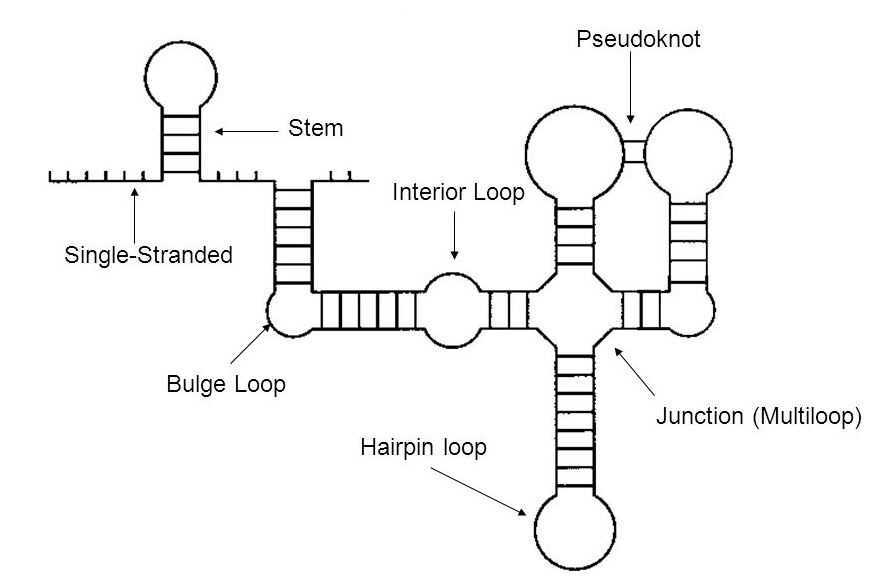
\includegraphics[width=\textwidth]{../img/secondary_structure}
\caption{Príklad nakreslenia sekundárnej štruktúre RNA. \cite{Eddy04}}
\label{obr01:secstru}
\end{figure}


\indent Zmyslom terciárnej štruktúry je popísať presné rozloženie jednotlivých atómov v trojdimenzionálnom priestore za pomoci koordinátov. V našej práci je hlavným cieľom tieto koordináty určiť za predpokladu znalosti primárnej sekvencie a terciárnych štruktúr ďalších RNA molekúl, ktoré sa pokúšame pri predikcii použiť ako vzory. 


\indent Kvarciárna štruktúra RNA popisuje vzťahy medzi celými molekulami RNA -
napríklad interakcie medzi jednotlivými molekulami RNA v ribozómoch \cite{Noller84} a taktiež vzťahy medzi RNA a molekulami bielkovín.

\section{Význam a získavanie terciárnej štruktúry}
Štruktúra RNA priamo súvisí s funkciou, ktorú vykonáva.Tvar štruktúry \ref{obr02:ecoli} určuje, ktoré enzýmy sa na ňu dokážu pripájanať a prípadne ju modifikovať a s ktorými bielkovinami a nukleovými kyselinami sa dokáže viazať. Bolo preukázané, že váčšina časti RNA štruktúry, ktoré sú schopné sa viazať s inými molekulami nie sú súčasťou žiadneho base pair-u a teda sú v sekundárnej štruktúre označené ako nespárované \cite{Schudoma10}. Zmena
terciárnej štruktúry, ktorá vedie ku strate pôvodnej funkcie molekuly, sa nazýva denaturácia.

%daj tu obrázok
\begin{figure}%[p]\centering
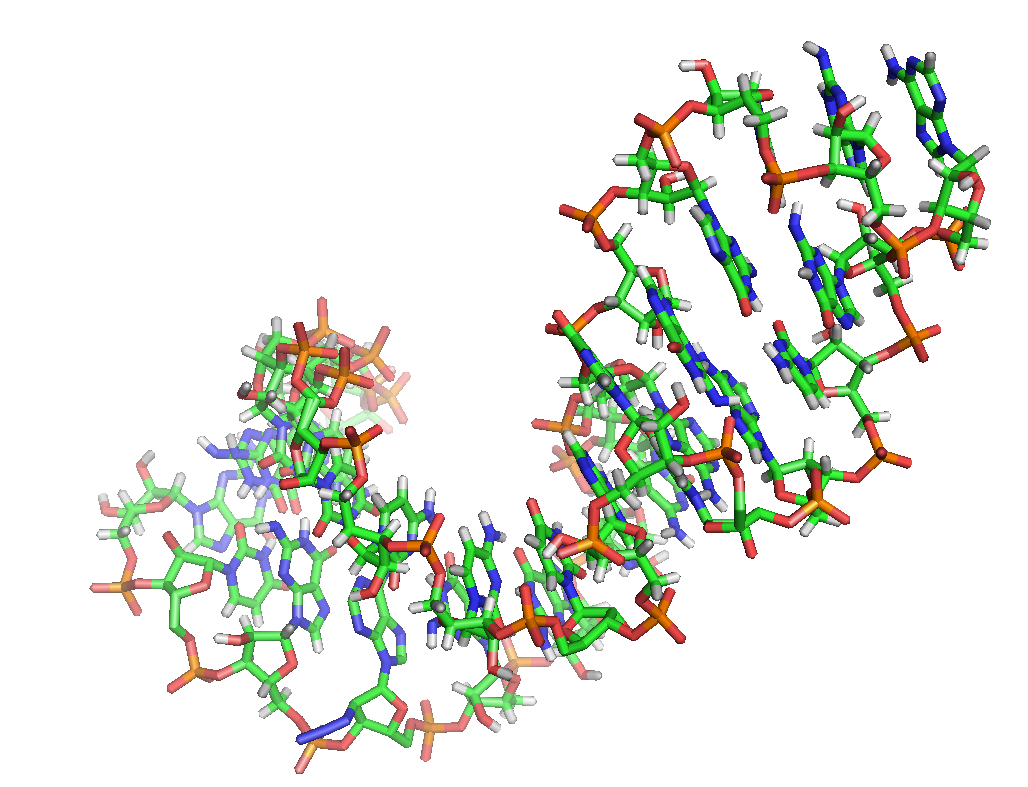
\includegraphics[width=\textwidth]{../img/ecoli_rna_example}
\caption{Príklad terciárnej štruktúry RNA nacházajúcej sa v baktérii  escherichia coli.}
\label{obr02:ecoli}
\end{figure}



\indent 
Bolo vyvinutých viacero experimentálnych metód, pomocou ktorých môžeme získať terciárnu štruktúru RNA \cite{Felden07}:
\begin{itemize}
\item metódy s vysokou presnosťou
\begin{itemize}
\item X-ray crystallography
\item Cryo-electron microscopy 
\item Nuclear Magnetic Resonance (NMR) spectroscopy
\end{itemize}
\item metódy s nižšou presnosťou
\begin{itemize}
\item Mass spectrometry
\item Chemical probing
\item Thermal denaturation
\item RNA engineering
\end{itemize}
\end{itemize}


\indent X-ray crystallography (rentgenova kryštalografia) funguje principiálne tak, že sa molekula najprv zkryštalyzuje a následne sa nasvieti rentgenovým lúčom. Z kryštálu je lúč odrazený a pritom rozdelený na viacero lúčov. Zmeraním týchto uhlova intenzity odrazených lúčov je následne možné určiť pozície jednotlivých atómov v molekule. Momentálne je to jesna z najpoužívanejších metód na získanie mnohých makromolekulárnych štruktúr. Rozlíšenie získanej štruktúry sa pohybuje okolo 2.0 Å. \ref{obr03:x-ray}


\begin{figure}%[p]\centering
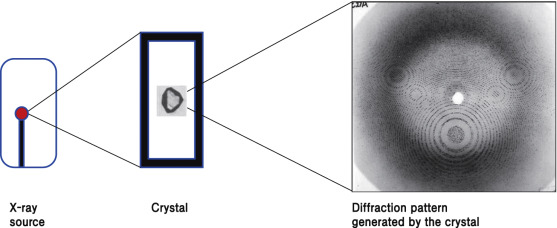
\includegraphics[width=\textwidth]{../img/x-ray}
\caption{Princíp rentgenovej kryštalografie. \cite{Ryu17}}
\label{obr03:x-ray}
\end{figure}


\indent Cryo-electron microscopy metóda využíva zmrazenie molekuly v substancií, ktorá je následne pozorovaná elektrónovým mikroskopom. Princíp metódy je známy približne od roku 1970, ale až donedávna pomocou nej nebolo možné získať tak presné vysledky, ako pomocou rentgenovej kryštalografie. Na druhej strane dĺžka skúmanej štruktúry nie je pri tejto metóde tak limitujúcim faktorom. V roku 2017 bola udelená nobelová cena za chémiu  J. Dubochetovi, J. Frankovi a  R. Hendersonovi za vyvinutie metódy, ktorou sa dá získať atómová štruktúra molekuly s vysokým rozlíšením.


\indent Metóda Nuclear Magnetic Resonance je založená na pôsobení statického magnetického poľa na jadrá atómov v molekule. Je vhodná hlavne na získavanie kratších štruktúr.


\indent Experimentálne prístupy sa od seba navzájom líšia presnosťou výsledku, dĺžkou štruktúry s ktorou sú schopné pracovať, ale ich hlavnám problémom je, že sú stále časovo náročné a drahé. Pretože získanie primárnej štruktúry RNA a proteinov je oveľa ľahšia úloha, začali byť skúmané aj možnosti, ako predikovať sekundárnu a terciárnu štruktúru za pomoci počítača, čomu sa budeme v našej práci venovať.
\chapter{Metódy výpočetnej predikcie}
Cieľom výpočetnej predikcie RNA štruktúry je dokázať algoritmicky modelovať terciárnu alebo sekundárnu štruktúru na základe znalosti primárnej sekvencie RNA molekuly. Pri takejto predikcii je dôležité, aby sme dostali čo najpresnejší výsledok v porovnaní s experimentálnymi metódami, a zároveň aby výpočtové nároky a čas boli výrazne nižšie, než v prípade experimentálnej rezolúcie štruktúry. Aby malo zmysel sa pokúšať o predikciu štruktúry zo sekvencie potrebujeme vedieť, že terciárna a teda aj sekundárna štruktúra je do veľkej miery jednoznačne určená štruktúrou primárnou.  


\indent Túto otázku môžeme zodpovedať vďaka znalostiam zo skladania (foldingu) proteínov, ktorých výskumu sa venovalo viacej úsilia. Platí, že skladanie bielkovín a RNA prebieha veľmi podobne, a preto poznatky o štruktúrach a sekvenciách bielkovín môžeme použiť aj pri RNA. \cite{Moore99} 


\indent  Existujú dve hlavné pozorovania, ktoré nám umožnujú štruktúry makromolekúl modelovať  \cite{Jenny09}:
\begin{itemize}
\item Štruktúra proteínu je unikátne určená sekvenciou aminokyselín.
\item Štruktúra sa zachováva aj pri určitých zmenách v sekvencii, a teda platí, že napriek odlišnosti v sekvenciách sú štruktúry veľmi podobné. Je to spôsobené tým, že počas evolúcie štruktúra stále plnila podobnú úlohu, a preto sa jej tvar nemenil aj napriek mutáciám sekvencie. Vďaka rozširujúcej sa databáze makromolekúl (Protein Data Bank) boli získané vzťahy určujúce, aká musí byť podobnosť rovnako dlhých sekvencií, aby sme mohli predpokladať, že aj ich štruktúry sú podobné. Tento vzťah zobrazuje obrázok  \ref{obr01:aln-zones}.
\end{itemize}

\begin{figure}%[p]\centering
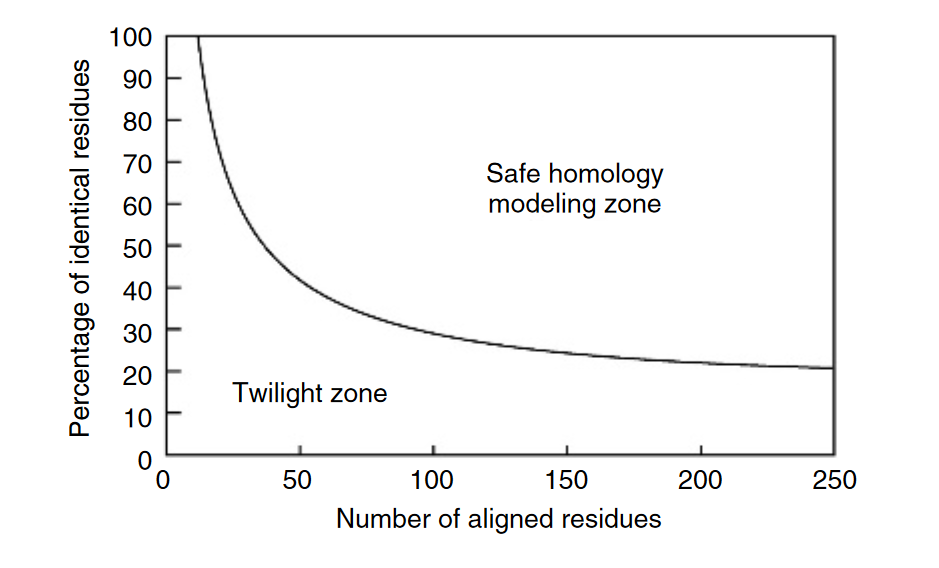
\includegraphics[width=\textwidth]{../img/zones_of_aln}
\caption{Vzťah dĺžky štruktúr a percentuálneho pomeru identických residuí v sekvenciách určujúce predpoklad, že štruktúry takýchto sekvencií sú podobné. \cite{Jenny09}}
\label{obr01:aln-zones}
\end{figure}

\section{Ab initio predikcia}
Pri ab initio predikcii štruktúry vychádzame iba z primárnej sekvencie a chemicko-fyzikálnych vlastností, vďaka ktorým sa v reálnom svete štruktúra skladá do stabilného tvaru. Algoritmus postupne vytvára kandidátske štruktúry tak, že sa snaží minimalizovať funkciu predstavujúcu voľnú energiu (energia, ktorá je ľahko dostupná v systéme). Následne z takto vygenerovaných kandidátov musí vybrať najprirodzenejšiu štruktúru. Najväčším problémom tohoto prístupu je mnoho lokálnych miním vo funkcii predstavujúcej voľnú energiu, a preto aj výpočetná zložitosť.


\indent  Tieto komplikácie sa dajú čiastočne riešiť viacerými spôsobmi. Jedna cesta je zvýšiť výpočetný výkon - použitie superpočítača, alebo distribuovať výpočet na mnoho výpočetných staníc. Ďalšia je pokus o zmenšenie vyhľadávacieho priestoru a efektívnejšie vyhľadávať kandidátske štruktúry. Jedna metóda je označovaná ako coarse-grained reprezentácie, kde nie sú reprezentované všetky atómy. Využívajú sa taktiež heuristické a pravdepodobnostné metódy na zmenšienie prehľadávaného priestoru.


\indent  Stále však platí, že takáto metóda je pre dlhšie štruktúry nepoužiteľná. Napriek tomu, že súšasný state-of-the art umožňuje predikovať štruktúry celkom presne, s rastúcou dĺžkou sekvencie neúmerne rastie výpočetná náročnosť. Ako príklad uvedieme pokus predikovať štruktúru dlhú 112 nukleotidov, pričom výsledná štruktúra sa líšila od experimentálne získanej len minimálne, výpočet však stál viac ako 100 000 hodín CPU.  \cite{Qian2007}


\section{Knowledge based de novo predikcia}
Princíp tohoto typu predikcie je veľmi podobný ako ten v ab initio metóde, ale namiesto samplovania možných usporiadaní atómov používa knižnicu krátkych úsekov štruktúry (väčšinou dĺžky 2-5 nukleotidov). Algoritmus následne vytvára kandidátske štruktúry tým, že kombinuje jednotlivé krátke úseky štruktúr z knižnice do kandidátskych štruktúr, a takisto minimalizuje voľnú energiu modelu. Výhodou je hlavne zrýchlené generovanie kandidátskych štruktúr oproti ab iniio predikcii. Aj tak je však predikovanie dlhých štruktúr príliš pomalé. Mnohé nástroje preto umožňujú vložiť sekundárnu štruktúru predikovanej sekvencie, a tak zmenšiť prehľadávaný priestor. 

\indent Ďalší spôsob ako znížiť prehľadávaný priestor, je použitie internej reprezentácie štruktúry. V prípade, že atómy reprezentujeme súradnicami v trojdimenzionálnom priestore, ich síce viem dobre zobraziť, ale takáto reprezentácia má 3*počet \_átomov stupňov voľnosti. Výhodnejšie je štruktúru reprezentovať napríklad pomocou reprezentácie uhlov medzi nukleotidmi.  \ref{obr02:reptesentation}


\begin{figure}%[p]\centering
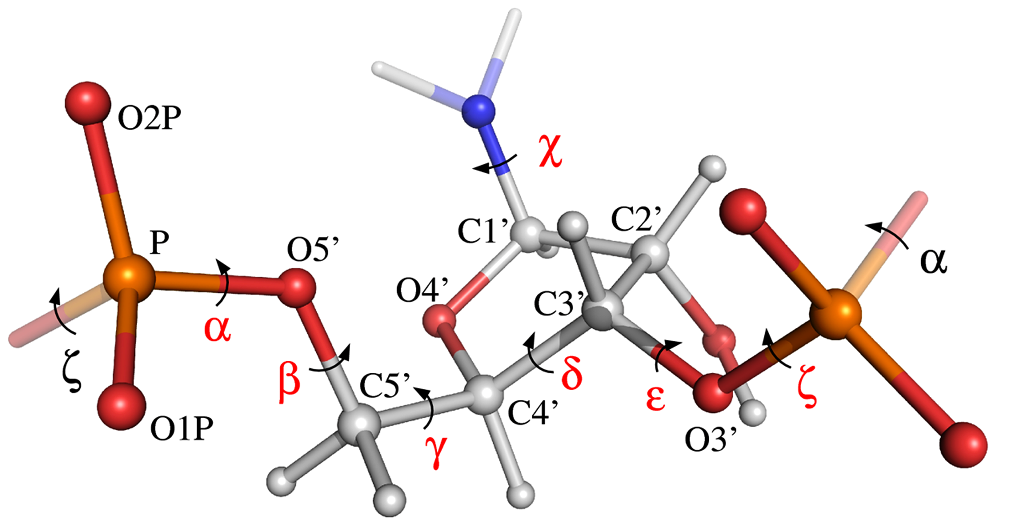
\includegraphics[width=\textwidth]{../img/str_reprezentace_uhly}
\caption{Reprezentácia RNA fragmentu pomocou siedmych uhlov. \cite{Frellsen09} }
\label{obr02:reptesentation}
\end{figure}


\indent Nástroj FARFAR \cite{Das10}, ktorý používame v našej predikcii, patrí tiež medzi knowledge based modelovacie metódy.


\section{Alignment sekvencií}
Zarovnanie dvoch sekvencií slúži na získanie informácie o tom, či sú dané sekvencie nejako evolučne, štrukturálne, alebo funkčne príbuzné. Existuje viacero druhov algoritmov zarovnania - napríklad jednoduchý dot plot vhodný na jednoduchú vizualizáciu zarovnania, heuristické metódy ako FASTA a BLAST určené na čo najrýchlejšie porovnanie sekvencie s rozsiahlou databázou ďalších sekvencií, alebo metódy počítajúce najlepšie zarovnanie určené skórovacím systémom za pomoci dynamického programovania.


\indent  V tejto práci budeme využívať semiglobálne zarovnanie pomocou algoritmu Needleman–Wunsch \cite{Needleman70}  implementovaného v programe EMBOSS \cite{Emboss}. Ako vstup algoritmus dostáva dve sekvencie dĺžiek m a n, ktoré chceme zarovnať, a hodnoty parametrov gap open (penalizácia v skóre za otvorenie medzery v zarovnaní) a gap extend (penalizácia v skóre za predĺženie medzery v zarovnaní). Algoritmus následne za pomoci dynamického programovania \ref{obr03:aln} vypočíta zarovnanie s najnižším skóre v čase aj priestore O(nm).  Výstupom algoritmu sú zarovnané sekvencie a skóre zarovnania. V zarovnaní na určitej pozícii môžu nastať tri prípady, a to zarovnanie dvoch rovnakých reziduí (match), zarovnanie dvoch odlišných reziduí (mismatch), a nakoniec zarovnanie rezidua na medzeru (gap) vloženú do druhej sekvencie. Nami používaná implementácia algoritmu nepenalizuje za medzery v zarovnaní nachádzajúce sa na začiatku alebo na konci zarovnania, preto je možné ňou zmysluplne zarovnať krátku štruktúru na časť oveľa dlhšej štruktúry.

\begin{figure}%[p]\centering
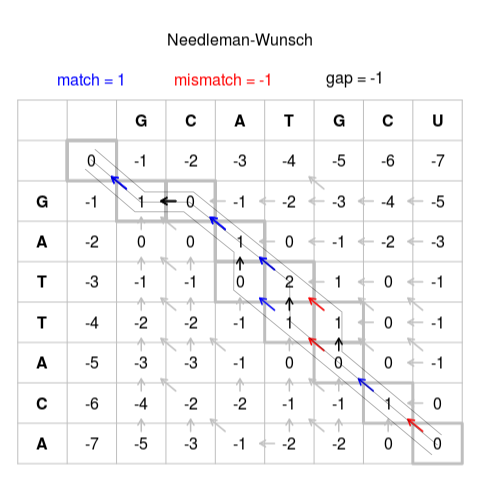
\includegraphics[width=\textwidth]{../img/needlemanwunsch}
\caption{Needleman–Wunsch algorithm (2014) Wikipedia dostupné na \url{https://en.wikipedia.org/wiki/Needleman–Wunsch\_algorithm} 27.05.2019. Príklad jedného z troch najlepších zarovnaní dvoch sekvencií: \newline GCATG-CU \newline G-ATTACA}
\label{obr03:aln}
\end{figure}


\indent Okrem globálneho poznáme aj presné lokálne zarovnanie vyriešené algoritmom Smith–Waterman \cite{Smith81}. Tento algoritmus pracuje taktiež na princípe dynamického programovania a vyhľadáva zarovnanie dvoch subsekvencií s najlepím skóre. Používa sa na nájdenie podobných regiónov medzi dvomi sekvenciami.


\section{Homológne modelovanie}
Tvrdenie zo začiatku kapitoly, ktoré hovorí, že štruktúra si zachováva podobný tvar aj napriek tomu, že jej sekvencia postupne mutuje, umožňuje zmysluplne predikovať štruktúru na základe vzoru.  


\indent Homológne modelovanie používa na modelovanie neznámej štruktúry zo sekvencie ešte jednu vzorovú sekvenciu (template), ktorej štruktúra je známa, teda získaná za pomoci nejakej experimentálnej metódy. Predikovanú štruktúru zvykneme nazývať cieľ (target).


\indent Prvým krokom je teda určenie vhodnej template štruktúry, pomocou ktorej budeme predikovať target štruktúru. Druhým krokom je globálne zarovnanie oboch sekvencií a získanie konzervovaných úsekov, teda úsekov, v ktorých by mali byť obe štruktúry veľmi podobné. Konzervované úseky môžu byť po nejakých úpravách prenesené do cieľovej štruktúry. Z princípu vyplýva, že čím podobnejšie sekvencie budú máť target a template štruktúry, tým viac konzervovaných úsekov bude existovať a tým jednoduchšia a presnejšia by mala predikcia byť.


\indent V treťom kroku musia byť dopredikované nekonzervované (chýbajúce úseky) cieľovej štruktúry. Existuje viacero prístupov. Jedným z nich je knižnica fragmentov, kde sa do chýbajúcej medzery v cieľovej štruktúre snažíme vhodne umiestniť fragment štruktúry z knižnice, ďalším je napríklad dopredikovanie medzery ab initio alebo de novo algoritmami.


\indent Takto hotový model sa nakoniec môže optimalizovať použitím algoritmu na minimalizovanie voľnej energie, alebo sa riešia kolízie medzi jednotlivými nukleotidmi.


\indent Hlavnou výhodou homológneho modelovania je, že je možné ho použiť na dlhé štruktúry. Problémom môže byť výber správnej template štruktúry a dopredikovanie nekonzervovaných úsekov. \ref{obr04:porovnanie}


\begin{figure}%[p]\centering
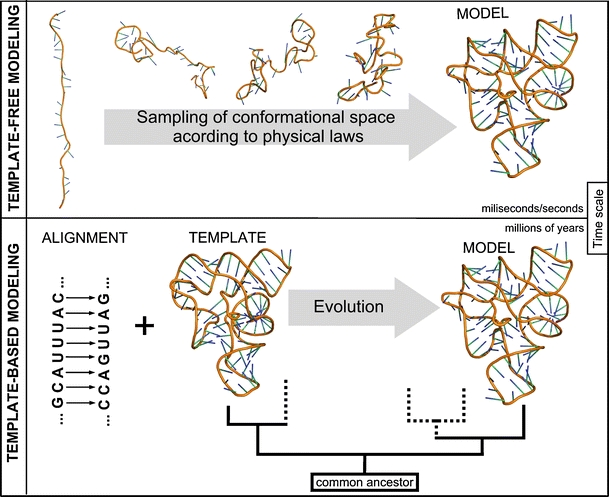
\includegraphics[width=\textwidth]{../img/template-vs-denovo}
\caption{Porovnanie princípu de novo a template based predikcie \cite{Rother11}}
\label{obr04:porovnanie}
\end{figure}


\section{Prehľad existujúcixh nástrojov}
Vďaka tomu, že počet dostupných primárnych sekvencií stále rastie rýchlejšie, ako počet experimentálne zistených terciárnych štruktúr, vzniklo mnoho nástrojov na predikciu terciárnej štruktúry RNA. \ref{tab01}


\begin{table}[b!]
\centering
\begin{tabular}{@{}lll@{}}
\toprule
Názov  & Info  & Referencia \\
\midrule
\begin{tabular}[c]{@{}l@{}}MacroMolecule\\ Builder\end{tabular} & komparatívny modeling RNA  & \cite{RNABuilder}   \\
ModeRNA & \begin{tabular}[c]{@{}l@{}}komparatívna predikcia s knižnicou \\ databázových fragmentov \\ na predikovanie medzier\end{tabular} & \cite{ModeRNA} \\
SimRNA & \begin{tabular}[c]{@{}l@{}}corase-grained model \\ s Monte Carlo samplingom štruktúr\end{tabular}    & \cite{SimRNA}  \\
FARFAR & knowledge based de novo prediktor & \cite{Das10} \\
RNAComposer & \begin{tabular}[c]{@{}l@{}}knowledge-based automatizovaná \\ predikcia štruktúry RNA \\  s využitím sekundárnej štruktúry\end{tabular} & \cite{Biesiada2016} \\
iFoldRNA & \begin{tabular}[c]{@{}l@{}}de novo predikcia RNA \\ založená na corase-grained model\end{tabular} & \cite{iFoldRNA} \\
\bottomrule

\end{tabular}

\caption{Prehľad niektorých programov určených na predikciu RNA s informáciou o type použitého algoritmu.}\label{tab01}

\end{table}


\section{ModeRNA}

ModeRNA je implementácia algoritmu komparatívneho modelovania RNA s ktorým sme porvnávali nami vyvinutý algoritmus. Je dostupná ako ModeRNA server a ponúka službu kompletnej predikcie submitovanej sekvencie (nájdenie vhodného template, zarovnanie sekvencií a vytvorenie modelu terciárnej štruktúry). Okrem toho je možné stiahnuť jej zdrojové kódy (Python) a nainštalovať a používať ju lokálne pre automatické hromadné spracovanie.


\indent Ako vstup ModeRNA požaduje zarovnanie  template a target sekvencií spolu so súradnicami jednotlivých atómov template štruktúry. Dodané zarovnanie ModeRNA nijako nemodifikuje a od jeho kvality a zvoleného template záleží výsldná presnosť predikcie. 
Zjednodušený algoritmus, ktorým ModeRNA predikuje štruktúru \cite{Rother11}: 

\begin{itemize}
\item Skopírovanie zarovnaných nukleotidov.
\item Substitúcia nukleotidov, ktoré boli zarovnané na iný nukleotid.
\item Modelovanie indelov vložením fragmentov štruktúr z knižnice obsahujúcej 131 316 fragmentov dĺžky 2-19 nukleotidov. ModeRNA najprv rýchlym filtrovaním podľa vzdialeností  prekrývajúcich sa atómov fragmentu a template-u vyberie 50 najvhodnejších kandidátov, pokúsi sa ich vložiť do medzery a pre každého kandidáta spočíta skóre. Následne vyberie jediného s najlepším skóre a vloží ho do medzery.
\item V prípade, že predikovaná štruktúra (backbone) nie je spojitá, ModeRNA sa ju pokúsi opraviť.
\end{itemize}


\section{FARFAR}

FARFAR je algoritmus de novo predikcie RNA implementovaný spolu s ďalšími bioinformatickými algoritmami a nástrojmi v balíčku Rosetta. My ho používame na predikovanie krátkych nekonzervovaných úsekov v našom algoritme.  


\indent Nástroj je schopný predikovať štruktúru iba z primárnej sekvencie. 


\indent Algoritmus pracuje tak, že nedeterministicky generuje kandidátske štruktúry, z ktorých vyberie tú s najnižšou voľnou energiou. Keďže sa jedná o algoritmus typu Monte Carlo, dve rôzne spustenia algoritmu môžu generovať rôzne výsledky a platí, že čím viac kandidátskych štruktúr vygenerujeme, tým viac máme šancí na vygenerovanie čo najlepšej štruktúry.


\indent Z pohľadu výkonnosti platí, že čím viac nukleotidov predikujeme (včetne tých pevne daných) tým predikcia dlhšie trvá. Pre presnejšiu predstavu sme urobili porovnanie, pričom sme predikovali nekonzervovaný úsek dlhý 9 nukleotidov. Pri zahrnutí zvyšných 129 konzervovaných nukleotidov do predikcie trvalo vygenerovanie jednej štruktúry približne 13 minút. Pri totožných podmienkach a parametroch s jedinou zmenou, a to, že sme do predikcie vybrali len 41 okolitých konzervovaných nukleotidov, trvala predikcia jednej kandidátskej štruktúry v priemere menej ako 6 minút.


\indent Očakávaná presnosť predikcie je priamo úmerná dĺžke neznámeho predikovaného úseku. Autori algoritmu uvádzajú, že pri predikcií štruktúr dĺžky 6 až 13 nukleotidov je priemerná RMSD menšia ako 2 Å. Pri štruktúrach dlhých 13-23 nukleotidov predstavovala priemerná RMSD už 6,5 Å.


\indent Je však takisto možné dať mu na vstup pdb súbor s koordinátami niektorých nukleotidov a zakázať mu tieto nukleotidy modifikovať. 
Takisto je možné mu dodať pdb súbor s nukleotidmi a dovoliť mu, aby ho algoritmus bral ako fixovaný kus štruktúry, ktorým môže ľubovoľne pohybovať oproti zvyšku štruktúry.
Posledná pre nás využiteľná možnosť je dodať algoritmu sekundárnu štruktúru target molekuly. Touto štruktúrou sa potom algoritmus pri predikcii riadi a zmenšuje sa tak prehľadávaný priestor.


\chapter{Algoritmus Trooper}

V tejto práci naväzujeme a ďalej vylepšujeme algoritmus Trooper, ktorý bol vytvorený v rámci mojej  bakalárskej práce na Matematicko-Fyzikálnej fakulte \cite{bc}. Preto v tejto kapitole uvedieme princípy fungovania a stav implementácie algoritmu tak, ako bol popísaný v bakalárskej práci.
Jedná sa o algoritmus založený na princípe homológneho modelovania, čo znamená, že predikujeme terciárnu RNA štruktúru na základe primárnej sekvencie molekuly označovanej ako target a známej terciárnej štruktúry a sekvencie inej RNA molekuly označovanej ako template.


\section{Kostra algoritmu}

V nasledujúcom zozname uvázdame postupnosť hlavných krokov algoritmu.\label{3-kostra}
\begin{enumerate}
\item Predpríprava a validácia vstupných súborov: template sekvencia, target sekvencia a štruktúra.
\item Alignemnt: Zarovnanie target a template sekvencií.
\item Sliding window: Algoritmus posuvného okienka na zarovnaní.
\item Treating indels: Vyriešenie medzier v zarovnaní. \label{3-indels}
\item Kopírovanie a mapovanie konzervovaných nukleotidov z target štruktúry do predikovanej template štruktúry. \label{3-map}
\item Vyčlenenie predikcie príliš dlhých medzier v target štruktúre.\label{3-sphere}
\item Príprava vstupu pre FARFAR.
\item Predikcia nekonzervovaných úsekov pomocou algoritmu FARFAR.
\item Zloženie predikovaných úsekov a dlhých medzier do finálnej štruktúry.
\end{enumerate}

\section{Popis algoritmu}
Ako vstup algoritmus dostane target sekvenciu a template sekvenciu aj štruktúru. Na výstupe očakávame terciárnu štruktúru target molekuly RNA.


\indent  Ako prvý krok algoritmus skontroluje, či sú sekvencia vo fasta súbore a štruktúra v pdb súbore rovnako indexované. Nukleotidy v pdb súbore sú očíslované, ale vo fasta súbore číslo nukleotidu odpovedá jeho pozícii v súbore. Kontrolujeme to prechodom cez pdb súbor tak, že indexom nukleotidu z pdb zaindexujeme do fasta súboru a typ nukleotidu musí byť v oboch súboroch na tejto pozícii zhodný. V prípade, že zhodný nie je, skúšame ešte posunúť fasta sekvenciu pridaním dummy nukleotidov na začiatok sekvencie (pre prípad, že by začiatok sekvencie v súbore chýbal). Ak sa nám nepodarí ani takýmto spôsobom dosiahnuť, aby sa typy nukleotidov v rovnakých indexoch zhodovali, označíme target za nevhodný pre predikciu a algoritmus končí neúspechom.


\indent V druhom kroku urobíme globálne zarovnanie (alignment) target a template sekvencií v programe Emboss Needle. Na vytvorené zarovnanie použijeme algoritmus posuvného okienka (sliding window) a pre každú pozíciu určíme percentuálnu mieru okolitých úspešne zarovnaných nukleotidov spadajúcich do okienka. V prípade, že získaná hodnota je vyššia ako parametrom určená hranica, označíme príslušnú pozíciu v zarovnaní ako konzervovanú. 


\indent V treťom kroku sa zaoberáme medzerami (indels), ktoré vznikli v terget alebo template sekvencii pri zarovnaní. Inak povedané, do oboch sekvencií mohol algoritmus zarovnania ľubovoľne vložiť medzery alebo na seba zarovnať nezhodujúce sa nukleotidy tak, aby získal zarovnanie s čo najlepším skóre \autoref{tab3.1}. 
To znamená, že medzery v inak konzervovanom úseku template sekvencie by vo výsledku nenechali miesto na doplnenie nukleotidov z target sekvencie zarovnaných oproti týmto medzerám z template sekvencie. 
Naopak, medzery v target sekvencii zarovnané oproti nukleotidom v template sekvencii v inak konzervovanom úseku by mohli spôsobiť medzeru v predikovanej štruktúre, nakoľko by sme z fragmentu konzervovanej štruktúry len odmazali nejaké nukleotidy a ničím ich nedoplnili. \autoref{obr3.1:indels}
Oba tieto problémy riešime tak, že nukleotidy v určitom okolí takýchto úsekov označíme za nekonzervované a budú dopredikované algoritmom FARFAR.
Taktiež označíme za nekonzervované tie nukleotidy, ktoré boli zarovnané na nezhodujúci sa typ nukleotidu. 

\begin{table}[b!]
\centering
\begin{tabular}{ccccc}
\toprule
Sekvencia  & konzervované  & nekonzervované & gap & gap \\
\midrule
tamplate  & G  & A & - & U \\
target  & G  & G & C & - \\
\bottomrule
\end{tabular}
\caption{Prehľad štyroch situácií, ktoré môžu nastať na každej pozícii v zarovnaní dvoch sekvencií.}\label{tab3.1}
\end{table}

\begin{figure}%[p]\centering
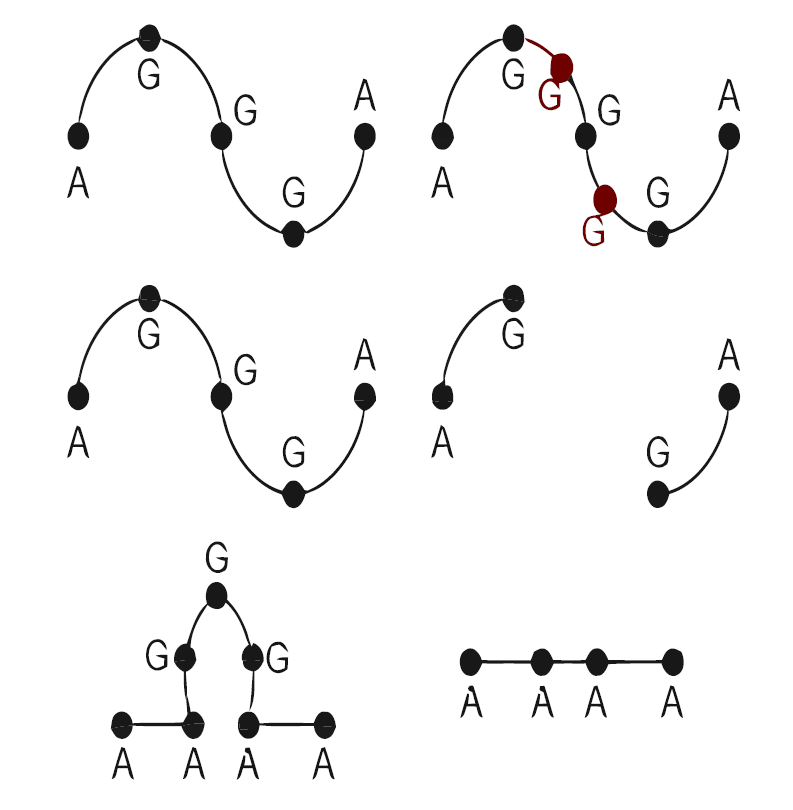
\includegraphics[width=\textwidth]{../img/aln-problems}
\caption{Problémy, ktoré môžu nasať v štruktúre pri vložení medzier do target alebo template časti zarovnania. Prvý riadok zobrazuje komplikácie pri pokuse vložiť nukleotidy (znázornene červenou farbou) do celistvej štruktúry (teda v zarovnaní boli pridané medzery do target sekvencie). Druhý riadok ukazuje opačný problém, a to vynechanie dvoch nukleotidov a roztrhnutie štruktúry (zodpovedá to vložením medzier do target sekvencie). Tretí riadok odpovedá rovnakej situácii ako druhý, ale odstránenie nukleotidov zo štruktúry nespôsobuje problém, pretože odstránené nukleotidy tvorili loop, ktorý môžeme bez problémov odobrať.}
\label{obr3.1:indels}
\end{figure}



\indent V štvrtom kroku skopírujeme konzervované časti template štruktúry do predikovanej target štruktúry. Vzhľadom na to, že v zarovnaní môžu byť rôzne vložené medzery do target aj template sekvencie, musíme premapovať indexy nukleotidov z template štruktúry tak, aby odpovedali nukleotidom, na ktorých miesto sú vložené v target sekvencii. Toto urobíme jednoducho vďaka informáciám zo zarovnania. Takto získame target štruktúru s medzerami, ktoré potrebujeme dopredikovať.


\indent V piatom kroku identifikujeme dlhé nekonzervované úseky a vyčleníme ich následnu predikciu do samostatných behov algoritmu FARFAR. 
Prvým dôvodom je, že takto sa môže FARFAR zamerať iba na predikciu dlhého úseku, a tým znížime celkovú výpočetnú náročnosť. Takisto môžeme zmeniť jeho parametry, ako napríklad zvýšiť počet samplovaných modelov, prípade zvýšiť celkový čas predikcie. 
Ďalším dôvodom, prečo dopredikovanie nekonzervovaných úsekov takto delíme je, že algoritmus FARFAR sa nedokáže dobre vysporiadať s predikciami príliš dlhých štruktúr, aj keď je časť nukleotidov pevne daná. Z tohto dôvodu rozdeľujeme dlhé štruktúry na úseky dĺžky 300 nukleotidov na základe ich poradia v sekvencii. Takéto delenie spôsobuje ďalší problém - nukleotidy, ktoré sú od seba vzdialené v sekvencii môžu byť blízko pri sebe v terciárnej štruktúre. 
Naše riešenie teda vyberie tieto dlhé nekonzervované úseky spolu s okolitými nukleotidmi, ktoré ležia v guli so stredom určeným úsečkou spájajúcou posledný konzervovaný nukleotid pred nekonzervovaným úsekom s prvým konzervovaným nukleotidom za nekonzervovaným úsekom vzhľadom na ich poradie v sekvencii. Polomer tejto gule je určený empiricky ako 0,75-násobok dĺžky úsečky, kedy by guľa mala obsiahnuť všetky relevantné nukleotidy. \autoref{obr3.2:sphere}

\begin{figure}%[p]\centering
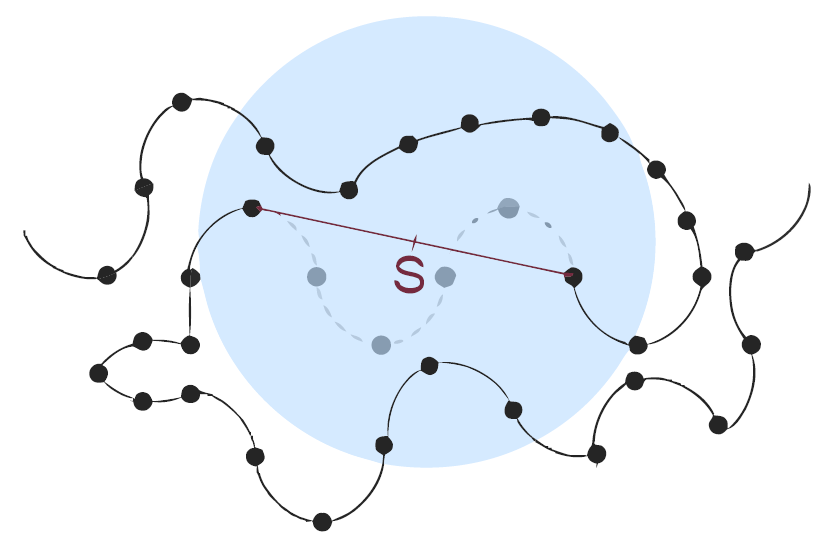
\includegraphics[width=\textwidth]{../img/sphere}
\caption{Schématické nakreslenie sféry so stredom v bode S, ktorý je stredom úsečky spájajúcej dva krajné konzervované nukleotidy medzery v štruktúre. Všetky nukleotidy, ktoré padnú do bledomodrej gule, budú použíte pri predikcii daného úseku.}
\label{obr3.2:sphere}
\end{figure}

\indent V šiestom kroku pripravíme vstupné dáta pre algoritmus FARFAR. To zahŕňa prípadné rozdelenie na úseky po 300 nukleotidov spomenuté v predchádzajúcom odstavci a prepísanie informácií o tom, ktoré nukleotidy sú pevne dané a ktoré treba dopredikovať do vstupného súboru. Takisto tu určíme parametre pre jednotlivé predikcie, ako napríklad počet vygenerovaných štruktúr.  


\indent
V siedmom kroku všetky takto pripravené časti predikcie spustíme a počkáme na výsledok. Toto je najpomalšia časť algoritmu, kedy FARFAR potrebuje čas minimálne pár hodín až niekoľko desiatok hodín, aby dokázal predikovať dlhšie nekonzervované úseky. Tie sú napriek tomu najväčšou slabinou nášho algoritmu, pretože podľa výsledkov získaných v bakalárskej práci platí, že čím dlhšie nekonzervované úseky sa nachádzajú v predikovaných štruktúrach tým je presnosť predikcie nižšia.


\indent V poslednom kroku najprv konvertujeme úseky z internej reprezentácie FARFARu do klasických pdb súborov a tie spojíme do výsledku.  


\section{Používané typy súborov}
V algoritme opakovane pracujeme s určitými typmi textových súborov. Sú to súbory s príponami fasta \textit{(uloženie sekvencie)}, secstr \textit{(uloženie sekundárnej štruktúry)}, pdb \textit{(uloženie terciárnej štruktúry)} a aln \textit{(uloženie zarovnania dvoch sekvencii)} \autoref{obr3.25:files}.

\begin{figure}%[p]\centering
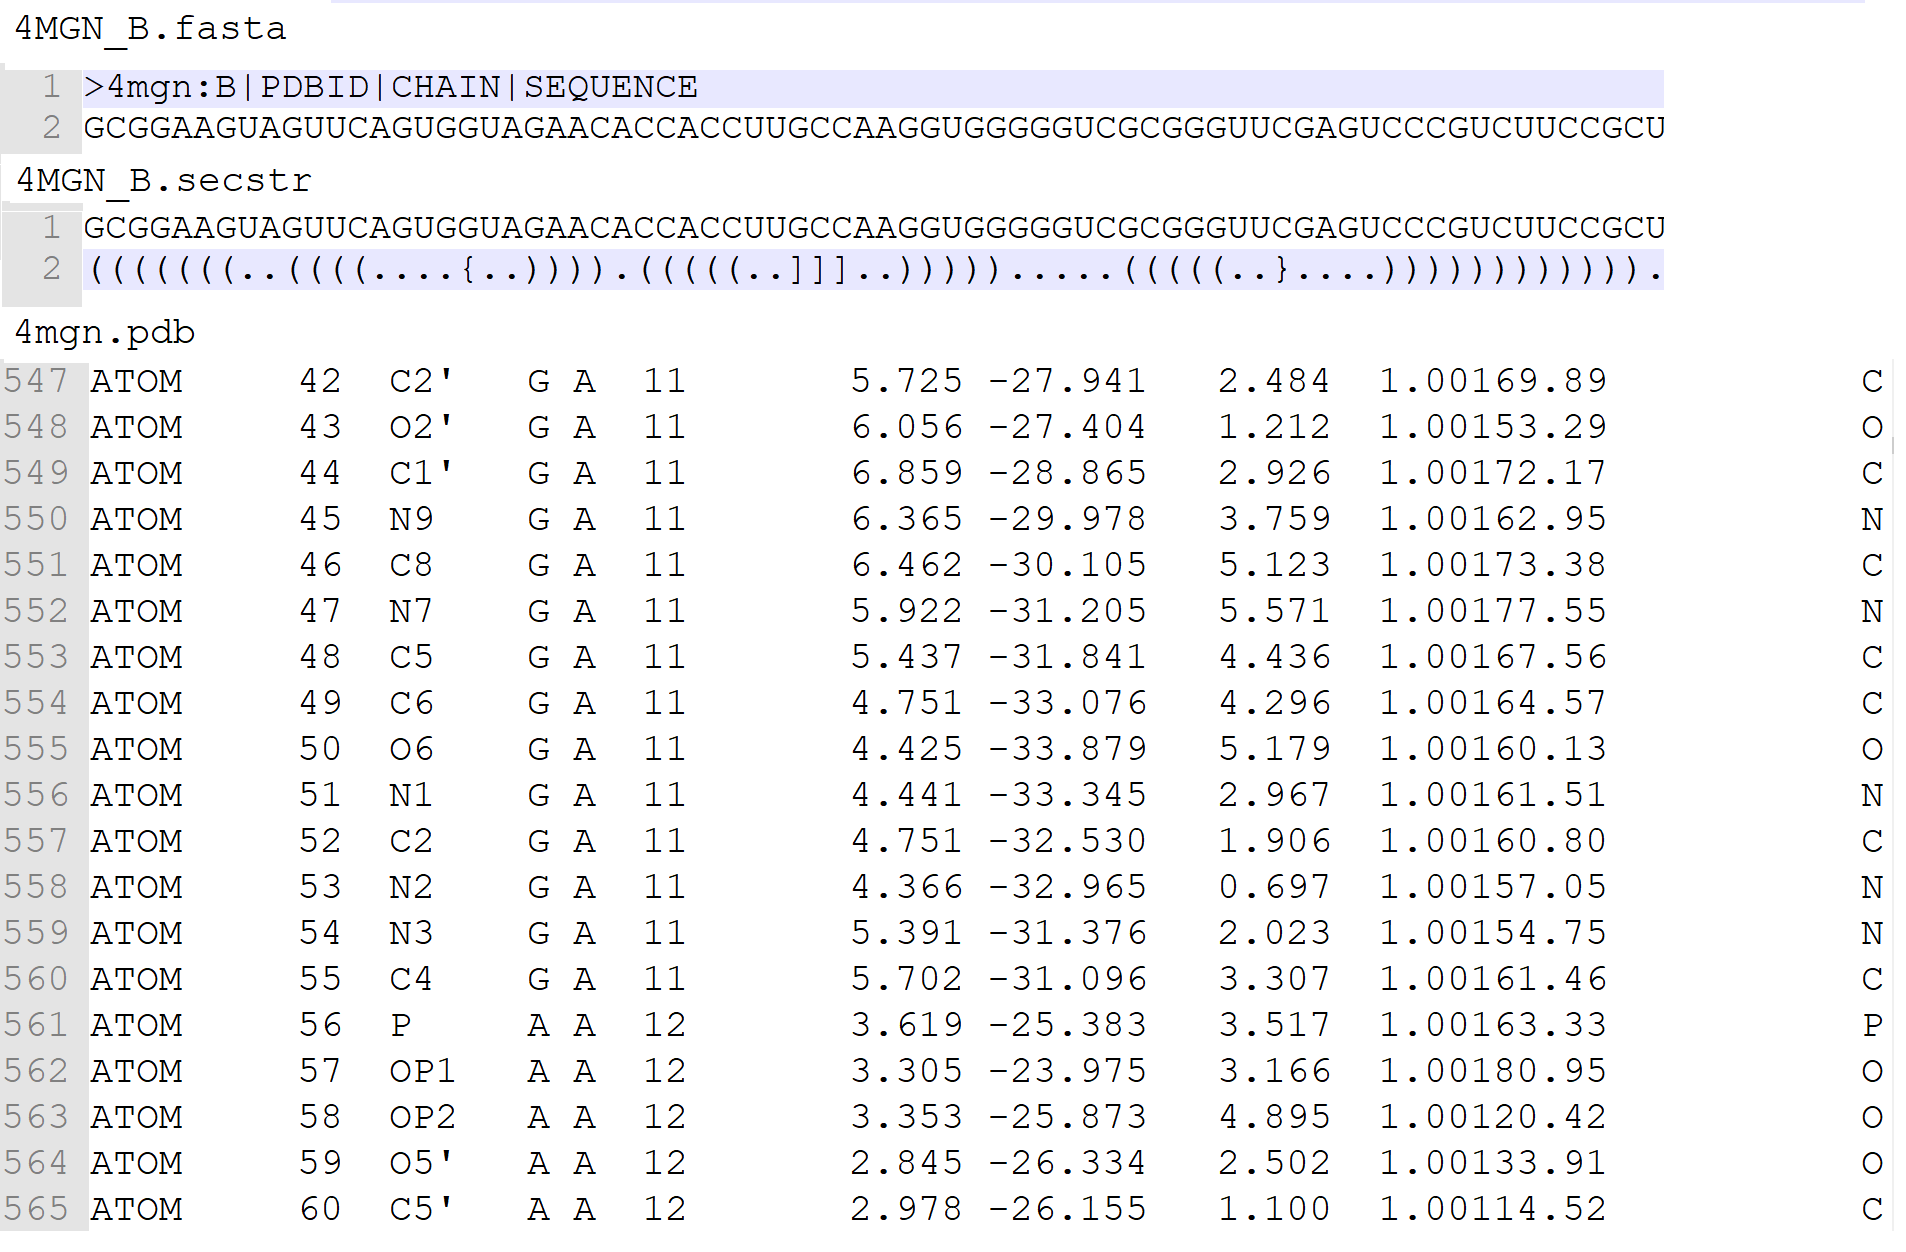
\includegraphics[width=\textwidth]{../img/files}
\caption{Na obrázku vidíme zhora nadol príklady súborov fasta, secstr a pdb pre molekulu 4mgn.}
\label{obr3.25:files}
\end{figure}

\indent Súbory typu fasta slúžia na ukladanie sekvencií. Pozostávajú z dvoch riadkov, v prvom je identifikátor sekvencie pozostávajúci z jej názvu a chain-u (jedna sekvencia máva  často viacero chains) a v ďalších riadkoch sú za sebou zoradené jednotlivé nukleotidy \textit{A, C, G, U}. V prípade, že je nejaký nukleotid v rade neznámy, bežne sa namiesto jeho typu úvádza písmeno \textit{N} alebo \textit{X}.


 \indent Súbory secstr nám slúžia na ukladanie informácií o sekundárnej štruktúre molekuly. Sú tvorené kombináciou rôznych typov zátvoriek, ktoré popisujú sekundárnu štruktúru tak, že medzi nukleotidmi odpovedajúcimi zátvorkám existuje chemická väzba - takéto dva nukleotidy sa tiež nazývajú base pair. Z toho vyplýva, že sa v terciárnej štruktúre budú nachádzať blízko pri sebe. Bodka v sekundárnej štruktúre znamená, že nukleotid netvorí base pair so žiadnym ďalším nukleotidom. Rôzne typy zátvoriek  ako \textit{[] , \{\}, <>} reprezentujú pseudouzly \cite{dbnotation}.


\indent Súbory typu pdb uchovávajú okrem iného informácie o jednotlivých atómoch molekuly. V každom riadku sú uložené informácie o presných koordinátoch atómu v 3D priestore, typ atómu vrámci nukleotidu, chain do ktorej atóm patrí a index nukleotidu, ktorému patrí. PDB súbory často nie sú kompletné, chýbajú v nich atómy alebo celé nukleotidy. Takisto sa stáva, že indexy nukleotidov v pdb súboroch a fasta súboroch nesúhlasia. Táto nekonzistentnosť medzi súbormi, alebo chýbajúce časti pdb súborov sťažujú ich algoritmické spracovanie.


\indent Súbory s príponou aln označujú výstup zarovnania dvoch sekvencií z programu EMBOSS Needle. Súbor obsahuje presné zarovnanie sekvenciií, skóre zarovnania, percentuálny pomer medzier v zarovnaní (gaps) a percentuálny pomer korektne zarovnaných nukleotidov označený ako similarity. 


\section{Popis implementácie}
Algoritmus bol implementovaný prevažne v programovacom jazyku Python 2.7. s využitím knižnice BioPython, ktorá zjednodušuje prácu so štandardnými súbormi používanými v bioinformatike, ako napríklad pdb a fasta. Okrem toho sme použili bash scripty na manipuláciu so súbormi a spustenie predikcie vo FARFAR.


\indent Algoritmus bol rozdelený na tri časti. Prvá pozostávala zo spustenia predikcie dopredu pripravenej target-template dvojice molekúl na lokálnom PC s operačným systémom Windows. To obsiahlo algoritmus  po siedmy krok, teda bola pipravená target štruktúra do stavu, kedy treba dopredikovať nekonzervované úseky algoritmom FARFAR. Následne boli takto pripravené vstupy pre FARFAR skopírované na servery organizácie Metacentrum používajúce operačný systém unixového typu s dávkovým spracovaním úloh. Vďaka tomu, že predikcie nekonzervovaných úsekov v rámci jednej molekuly sú na sebe nezávislé a tiež predikcie molekul medzi sebou sú nezávislé, môžeme predikcie nekonzervovaných úsekov algoritmom FARFAR paralelizovať. To je veľmi dôležité, pretože de novo predikcia nekonzervovaných úsekov bola najdlhšie trvajúca časť algoritmu a predikcia jednej štruktúry mohla obsahovať niekoľko takýchto de novo predikcií.  Po skončení FARFAR predikcií nekonzervovaných úsekov boli výsledky skopírované späť na lokálny PC a tam boli v treťom kroku vyhodnotené výsledky. 


\indent Časová náročnosť celého algoritmu je závislá hlavne na nekonzevovaných úsekoch, ktoré treba predikovať. Časť predikcie po algoritmus FARFAR beží v rádoch desiatok sekúnd. Pre FARFAR sme okrem pár problémových predikcií používali obmedzenie predikcie časom 24 hodín, prípadne 100 štruktúr. To znamená, že FARFAR buď stihne do 24 hodín namodelovať 100 modelov štruktúr, alebo s modelovaním skončí predčasne po 24 hodinách a výsledkom bude počet modelov štruktúr, ktoré sa mu do 24 hodín podarilo namodelovať. Z namodelovaných štruktúr sa vyberie tá s najmenšou voľnou energiou. Počet a kvalita kandidátskych štruktúr, ktoré za tento čas algoritmus stihne vygenerovať, záleží na počte nekonzervovaných úsekov, ich dĺžke (problematické sú hlavne dlhé nekonzervované úseky) a dĺžke celej predikovanej štruktúry včetne konzervovaných nukleotidov. Záverečné získanie výsledkov a porovnanie s experimentálne získanými štruktúrami prebieha opäť v rádoch desiatok sekúnd.


\section{Pseudokód}\label{kap3:pseudocode}
V tejto sekcii uvádzame pseudokód algoritmu Trooper v stave po bakalárskej práci. Premenné  začínajú malým písmenom, názvy metód veľkým písmenom. Pseudokód ignoruje prácu s datami a znaky \textit{[]} za premennou znamenajú, že premenná nahrádza množinu pdb súborov. Pseudokód nám bude ďalej v práci slúžiť aj na to, aby sme sa vedeli na jendotlivé metódy v prípade potreby odkazovať.


\lstset{numbers=left, numberstyle=\tiny, stepnumber=1, numbersep=5pt}
\begin{lstlisting}
Main(fastaTarget, fastaTemplate, pdbTemplate)
{
   CheckTemplateMapping
      (fastaTemplate, pdbTemplate)
   alignment := Align
      (fastaTarget, fastaTemplate)
   alignment1 := UseSlidingWindow
      (alignment)
   alignment2 := ProcessGaps
      (alignment1)
   conservedParts := CopyConservedParts
      (alignment2, pdbTemplate)
   mappedConservedParts := MapConservedParts
      (conservedParts, alignment2)
   longParts[] := ProcessLongUnconservedParts
      (mappedConservedParts)
   shortParts[] := ProcessShortUnconservedParts
      (mappedConservedParts)
   predictedParts[] := PredictUnconservedParts
      (longParts[], shortParts[])
   finalModel := ConnectPredictedParts
      (predictedParts)
}

CheckTemplateMapping(fasta, pdb)
{
   foreach res in pdb
   {
         if (fasta[res[id]] != res[type])
         ERROR: Input needs manual editing!
         EXIT PROGRAM	
   }
}

Align(fastaTarget, fastaTemplate)
{
   string alignment := CallEmbossAln
      (fastaTarget, fastaTemplate)
   return EditAlignmentFormat(alignment)
}

SlidingWindow(alignment, windowLength, minimalLimit)
{
   hL = windowLength DIV 2	
   foreach nucleotide in alignment 
   {
      check if in [nucleotide[id]-hL, nucleotide[id]+hL]
      is less than minimalLimit conserved nucleotides
      if so mark nucleotide as unconserved
   }		
   return modifiedAln  
}

ProcessGaps(alignment, cutoff)
{
   foreach gap in alignment 
   {
      alignment := mark "cutoff" nucleotides from 
         both sides of the gap as unconserved 
   }	
   return alignment
}

CopyConservedParts(alignment, pdb)
{
   conservedParts = ""
   foreach nucleotide in pdb 
   {
      if (IsConserved(nucleotide, alignment))
         conservedParts += nucleotide
   }
   return conservedParts
}

MapConservedParts(conservedParts, alignment)
{
   map nucleotide id's from current state (nc with
   id x corresponds to x-th nc in template fasta) to 
   state where nc id correctly corresponds to 
   nucleotide in target fasta 
   return modifiedConservedParts
}

ProcessLongUnconservedParts
   (conservedParts, ncAvarageLength, minLengthGapLimit)
{
   longParts = []
   foreach gap in conservedParts
   {
      if length(gap) <= minLengthGapLimit
         continue
      startNc := conserved nucleotide before gap
      endNc := conserved nucleotide after gap
      ph="phosphor"
      s := FindMiddle(startRes[ph], endRes[ph])
      p := length(gap) * ncAvarageLength / 2
      ncsInSphere := all nucleotides inside sphere(p, s)
      preparedPart := PrepareCorectFormatForFARFAR
         (ncsInSphere)
      longParts[] += preparedPart
   }
   return longParts[]
}

ProcessShortUnconservedParts
   (conservedParts, lengthOfSection, maxLengthGapLimit)
{
   createdSections = []
   createdSections[] = divide "conservedParts" into 
      sections with length of "lengthOfSection"
   preparedSections = []
   foreach section in createdSections[]
   {
      preparedSections[] += PrepareCorectFormatForFARFAR
         (section, maxLengthGapLimit)
   }
   return preparedSections[]
}

PredictUnconservedParts(lgUnconsPts[], shUnconsPts[])
{
   predictedParts = []
   allParts := lgUnconsPts[] + shUnconsPts[]
   foreach input in allParts
   {
      predictedParts[] += CallFARFAR(input)
   }
   return predictedParts[]	
}

ConnectPredictedParts(predictedParts[])
{
   connect all conserved and predicted nucleotides 
   into single file in case of duplicity
   (they are almost the same) choose only one 
}
\end{lstlisting}


\section{Časová zložitosť}
V tejto sekcii rozoberieme časovú zložitosť algoritmu ako reálnu, tak aj asymptotickú, ktorou sme sa v bakalárskej práci nezaoberali. Budeme na to potrebovať definovať premennú dĺžka molekuly \textit{l}, kedy budeme predpokladať, že všetky molekuly s ktorými pracujeme majú takúto dĺžku. 


\indent Asymtoticky zložitosť rozoberieme podľa jednotlivých metód pseudokódu:
 \begin{enumerate}
\item Main: hlavná metóda, ktorá len prevoláva ostatné metódy. \textit{O(1)}
\item CheckTemplatetMapping: Sekvenčný prechod cez fasta a pdb súbory template molekuly: \textit{O(l)}
\item Align: zarovnanie target a template sekvencie: \textit{O($l^2$)}
\item Sliding window: sekvenčný prechod zarovnaním \textit{O(l)}
\item ProcessGaps: sekvenčný prechod zarovnaním \textit{O(l)}
\item CopyConservedParts: sekvenčný prechod zarovnaním \textit{O(l)}
\item MapConservedParts: Je možné to urobiť dvomi sekvenčnými prechodami v čase O(l), implementované to však je dosť nešikovne v čase \textit{O($l^2$)} 
\item ProcessLongUnconservedParts: sekvenčný prechod target sekvenciou \textit{O(l)}
\item ProcessShortUnconservedPairs: sekvenčný prechod target sekvenciou \textit{O(l)}
\item PredictUnconservedPairs: volanie algoritmu FARFAR. Čas považujeme za konštantný, pretože beh obmedzujeme na 1 deň \textit{O(1)}. Asimptotickú zložitosť nástroja sa nám nepodarilo dohľadať. 
\item ConnectUnconservedPairs: sekvenčný prechod napredikovanými úsekmi \textit{O(l)}
 \end{enumerate}

Celková asymptotická zložitosť nášho algoritmu (v prípade, že FARFAR obmedzíme na \textit{O(1)}) je  \textit{O($l^2$)}. 

\indent Keď sa pozrieme na reálny čas behu, najviac sa na ňom podieľa algoritmus FARFAR a to jedným  dňom, pri štruktúrach dlhých 50-500 nukleotidov. Príprava predikcie a následne spojenie a vyhodnotenie výsledkov zaberie pre jednu štruktúru dlhú 50-500 nukleotidov menej ako 1 minútu.


\section{Hlavné problémy algoritmu a jeho implementácie}
Najväčším problémom v našom algoritme, ktorý sme identifikovali na základe výsledkov bakalárskej práce, je predikcia dlhších nekonzervovaných úsekov \autoref{obr3.3:badPredictedRegion}. Preto by sme potrebovali minimalizovať takéto úseky, prípadne pomôcť algoritmu FARFAR zmenšiť prehľadávaný priestror pri generovaní kandidátskych štruktúr. To by potom mohlo pomôcť rýchlosti predikcie kandidátskych štruktúr FARFAR-om a zlepšiť jeho presnosť. Takisto by sme chceli do väčšej miery automatizovať predikciu, a urobiť ju uživateľsky prívetivejšou.

\indent Aby sme zlepšili problematické časti algoritmu a jeho implementácie navrhujeme niekoľko vylepšení ako algoritmu, tak aj implementácie. Tieto opatrenia popíšeme v nasledujúcich troch kapitolách a sú hlavným prínosom tejto práce. Tu uvádzame ich prehľad:
\begin{enumerate}
\item Algortimus predikcie
\begin{enumerate}
\item Pridanie predikcie sekundárnej štruktúry, ako medzikroku pri predikovaní terciárnej štruktúry.
\item Pridanie možnosti použiť viacero template molekúl pri predikcii jednej target molekuly.
\item Algoritmické vyhľadanie vhodnej template štruktúry.
\end{enumerate}
\item Implementácia
\begin{enumerate}
\item Presunúť celú predikciu na Metacentrum.
\item Predikcia prebehne bez manuálnych zásahov do procesu.
\item Vysporiadanie sa s chybnými pdb a fasta súbormi.
\end{enumerate}
\item Vyhodnotenie výsledkov
\begin{enumerate}
\item Porovnanie s nástrojom ModeRNA, ktorý tiež funguje na princípe komparatívneho modelovania.
\item Vyhodnotenie na všetkých dostupných kombináciach target-template párov, ktoré má zmysel predikovať, nakoľko v bakalárskej práci sme vybrali len niekoľko desiatok párov, na ktorých sme predikciu skúšali a vyhodnocovali výsledky.
\end{enumerate}
\end{enumerate}


\begin{figure}%[p]\centering
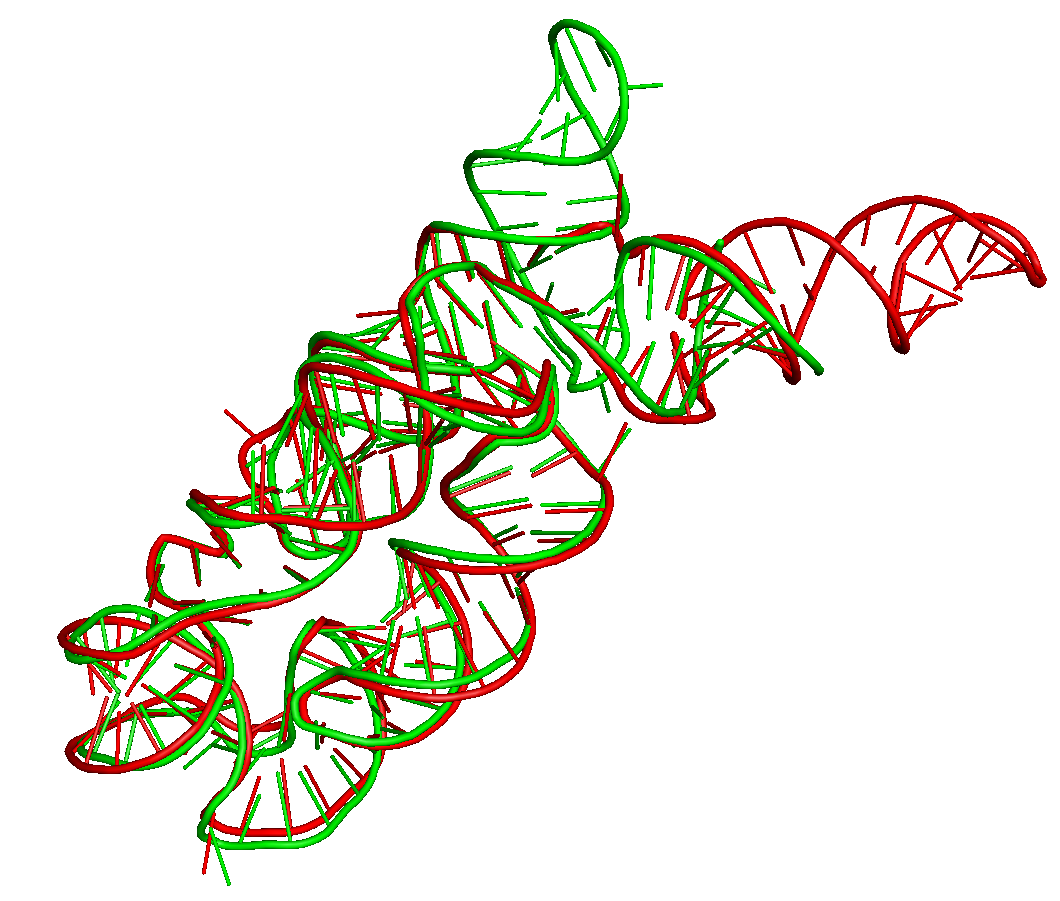
\includegraphics[width=\textwidth]{../img/badPredictedRegion}
\caption{Na obrázku vidíme zarovnanie experimenntálne získanej (3DIG) štruktúry a jej predikcie, napredikovanou našim algoritmom vytvoreným v bakalárskej práci. V pravej hornej časti obrázka vidíme, že algoritmu FARFAR sa nepodarilo správne napredikovať nekonzervovaný úsek.}
\label{obr3.3:badPredictedRegion}
\end{figure}

%%% Fiktivní kapitola s instrukcemi k PDF/A

\chapter{Formát PDF/A}

Opatření rektora č. 13/2017 určuje, že elektronická podoba závěrečných
prací musí být odevzdávána ve formátu PDF/A úrovně 1a nebo 2u. To jsou
profily formátu PDF určující, jaké vlastnosti PDF je povoleno používat,
aby byly dokumenty vhodné k~dlouhodobé archivaci a dalšímu automatickému
zpracování. Dále se budeme zabývat úrovní 2u, kterou sázíme \TeX{}em.

Mezi nejdůležitější požadavky PDF/A-2u patří:

\begin{itemize}

\item Všechny fonty musí být zabudovány uvnitř dokumentu. Nejsou přípustné
odkazy na externí fonty (ani na \uv{systémové}, jako je Helvetica nebo Times).

\item Fonty musí obsahovat tabulku ToUnicode, která definuje převod z~kódování
znaků použitého uvnitř fontu to Unicode. Díky tomu je možné z~dokumentu
spolehlivě extrahovat text.

\item Dokument musí obsahovat metadata ve formátu XMP a je-li barevný,
pak také formální specifikaci barevného prostoru.

\end{itemize}

Tato šablona používá balíček {\tt pdfx,} který umí \LaTeX{} nastavit tak,
aby požadavky PDF/A splňoval. Metadata v~XMP se generují automaticky podle
informací v~souboru {\tt prace.xmpdata} (na vygenerovaný soubor se můžete
podívat v~{\tt pdfa.xmpi}).

Validitu PDF/A můžete zkontrolovat pomocí nástroje VeraPDF, který je
k~dispozici na \url{http://verapdf.org/}.

Pokud soubor nebude validní, mezi obvyklé příčiny patří používání méně
obvyklých fontů (které se vkládají pouze v~bitmapové podobě a/nebo bez
unicodových tabulek) a vkládání obrázků v~PDF, které samy o~sobě standard
PDF/A nesplňují.

Další postřehy o~práci s~PDF/A najdete na \url{http://mj.ucw.cz/vyuka/bc/pdfaq.html}.

\chapter{Predikcia sekundárnej štruktúry}

Na zlepšenie rýchlosti a presnosti predikovania nekonzervovaných úsekov sme ako prvé opatrenie navrhli riešiť najprv jednoduchší problém, a to predikciu sekundárnej target štruktúry, a pomocou nej neskôr predikovať terciárnu štruktúru nekonzervovaných úsekov. To by malo viesť k zmenšeniu prehľadávaného priestoru pri generovaní kandidátskych štruktúr algoritmom FARFAR. Principiálne teda najprv komparatívnym modelovaním napredikujeme sekundárnu target štruktúru, a tú potom poskytneme ako vstup algoritmu FARFAR, ktorý ju použije pri predikcii terciárnej target štruktúry. Tento postup a jeho výsledky sme popísali aj v článku \cite{8218009}.

\section{Príprava dát}
Pretože algoritmus doplníme o komparatívne predikovanie sekundárnej štruktúry, nebude na vstupe potrebovať len sekvenciu target molekuly a terciárnu štruktúru spolu so sekvenciu template molekuly, ale aj sekundárnu štruktúru template molekuly. Sekundárnu štruktúru očakávame v dot-bracket notácii, ktorú sme popísali v druhej kapitole. Sekundárnu štruktúru by bolo možné získať z terciárnej template štruktúry aj počas predikcie, avšak v prípade, kedy si užívateľ chce dodať vlastnú sekundárnu štruktúru, je preňho výhodnejšie, keď je sekundárna štruktúra dodaná ako ďalší vstupný parameter.


\indent Získať dáta sme sa rozhodli ich určením z terciárnej štruktúry programom DSSR (Defining the Secondary Structures of RNA) zo software balíku x3DNA \cite{x3dna}. Na hromadné extrahovanie štruktúr sme si potom vytvorili dva krátke scripty, ktoré len prejdú všetky pdb súbory v databáze, spustia DSSR a uložia výsledok. DSSR vytvára v sekundárnej štruktúre base-pairs vyznačené jednoduchými zátvorkami, ako aj pseudo uzly vyznačené hranatými zátvorkami \autoref{obr5.0}. Z dôvodov implementačných komplikácií a zladenia s algoritmom FARFAR sme sa rozhodli pracovať iba so sekundárnou štruktúrou označujúcou base-pairs, a preto pseudo uzly neberieme do úvahy.
\begin{figure}%[p]\centering
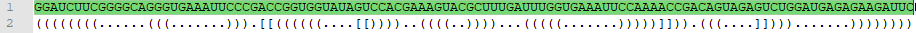
\includegraphics[width=\textwidth]{../img/dssr}
\caption{Príklad súboru sekundárnej štruktúry získanej progrmaom DSSR zo štruktúry terciárnej. V prvom riadku sú príslušné typy nukleotidov a v druhom riadku je samotná sekundárna štruktúra v  dot-bracket reprezentácii.}
\label{obr5.0}
\end{figure}

\section{Pseudokód}\label{kap5:pseudocode}
 Pseudokód algoritmu predikujúceho sekundárnu štruktúru spolu s integráciou do pôvodného algoritmu, ktorý vychádza z pseudokódu algoritmu Trooper v kapitole 3 (\autoref{kap3:pseudocode}).
\lstset{numbers=left, numberstyle=\tiny, stepnumber=1, numbersep=5pt}
\begin{lstlisting}
Main(fastaTarget, fastaTemplate
        , secStrTemplate, pdbTemplate)
{
   CheckTemplateMapping
      (fastaTemplate,pdbTemplate)
   alignment := Align
      (fastaTarget, fastaTemplate)
   alignment1 := UseSlidingWindow
      (alignment)
   alignment2 := ProcessGaps
      (alignment1)
   conservedParts := CopyConservedParts
      (alignment2, pdbTemplate)
   mappedConservedParts := MapConservedParts
      (conservedParts, alignment2)
   conservedPartsSecStr := CopyConservedPartsSecStr
      (alignment2, secStrTemplate)
   cleanedConservedPartsSecStr := CleanConservedPartsSecStr
      (conservedPartsSecStr, alignment2)
   mappedConservedPartsSecStr := MapConservedPartsSecStr
      (cleanedConservedPartsSecStr, alignment2)
   predictedSecStr := PredictUnconservedSecStr
      (mappedConservedPartsSecStr)
   longParts[] := ProcessLongUnconservedParts
      (mappedConservedParts, secStr)
   shortParts[] := ProcessShortUnconservedParts
      (mappedConservedParts, secStr)
   predictedParts[] := PredictUnconservedParts
      (longParts[], shortParts[])
   finalModel := ConnectPredictedParts
      (predictedParts)
}

CopyConservedPartsSecStr(alignment, secStr)
{
   conservedPartsSecStr = ""
   foreach nucleotide in secStr 
   {
      if (IsConserved(nucleotide, alignment) and
          CorrespondingPairIsConserved)
         conservedParts += nucleotide
   }
   return conservedParts
}

CleanConservedPartsSecStr(conservedPartsSecStr, aln2)
{
   remove base-pairs from conservedPartsSecStr, which 
   were aligned to gaps in target structure
}

MapConservedPartsSecStru(conservedPartsSecStr, alignment)
{
   map nucleotide id's from current state (nc with
   id x corresponds to x-th nc in template fasta) to 
   state where nc id correctly corresponds to 
   nucleotide in target fasta 
   return modifiedConservedSecStrParts
}

PredictUnconservedSecStr(mappedConservedPartsSecStr)
{
    input = Tuple(targetFasta, mappedConservedPartsSecStr)
    predictedSecstr+= CallRNAFold(input)
    return predictedSecstr
}

ProcessLongUnconservedParts
   (conservedParts, ncAvrgLength, minLenGapLimit, secStr)
{
   longParts = []
   foreach gap in conservedParts
   {
      if length(gap) <= minLenGapLimit
         continue
      startNc := conserved nucleotide before gap
      endNc := conserved nucleotide after gap
      ph="phosphor"
      s := FindMiddle(startRes[ph], endRes[ph])
      p := length(gap) * ncAvrgLength / 2
      ncsInSphere := all nucleotides inside sphere(p, s)
      secStrInSphere := all secstr pairs(ncsInSphere)
      ncsInSphere += add missing nucleotides from
         secStrInSphere, when second nucleotide from 
         pair is missing in ncsInSphere
      preparedPart := PrepareCorectFormatForFARFAR
         (ncsInSphere, secStrInSphere)
      longParts[] += preparedPart
   }
   return longParts[]
}
\end{lstlisting}


\section{Predikcia sekundárnej štruktúry}
Sekundárnu štruktúru predikujeme rovnakým spôsobom ako štruktúru terciárnu, teda komparatívnym modelovaním. Ako vstup potrebuje algoritmus dostať sekvenciu target molekuly, sekvenciu, sekundárnu  a terciárnu štruktúru template molekuly. 


\indent  Používame rovnakú template štruktúru ako pre terciárnu predikciu, a preto sa algoritmus predikcie sekundárnej štruktúry zhoduje s algoritmom predikcie terciárnej štruktury až po získanie konzervovaných úsekov v zarovnaní (teda metódu \textit{ProcessGaps}). Následne potrebujeme na zarovnanie namapovať sekundárnu template štruktúru. Tu musíme riešiť nasledujúcu situáciu: ak práve jeden nukleotid z base-pair z template sekvencie je zarovnaný na medzeru v target sekvencii a druhý je zarovnaný na nukleotid, musíme v sekundárnej template štruktúre preznačiť oba nukleotidy ako nespárované, inak by namapovaná sekundárna štruktúra bola neplatná \autoref{obr5.0}. Tiež to môžeme chápať tak, že sekundárnu štruktúru udržujeme stále správne uzátvorkovanú, čo znamená, že zátvorky rovnakého typu sa navzájom nekrížia, a máme stále rovnaký počet pravých aj ľavých zátvoriek v sekundárnej štruktúre.


\begin{figure}%[p]\centering
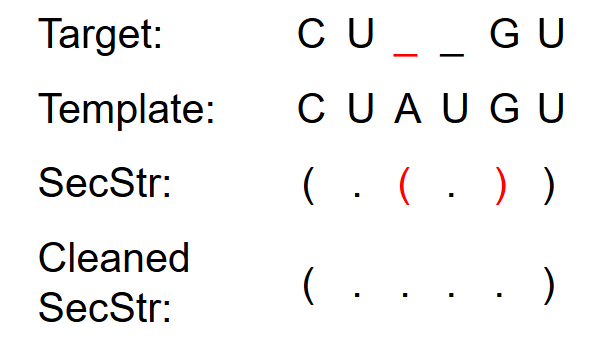
\includegraphics[width=\textwidth]{../img/cleanStr}
\caption{Príklad problému, ktorý môže nastať pri mapovaní sekundárnej štruktúry na zarovnanie. Z obrázku vidíme, že tretí a štvrtý nukleotid template štruktúry, sú zarovnané na medzery v target štruktúre. Sekundárna template štruktúra, ktorú potrebujeme namapovať na zarovnanú target štruktúru obsahuje base-pair tvorený tretím a piatym nukleotidom (vyznačené červenou farbou).  Z dôvodu, že tretí nukleotid template štruktúry je zarovnaný na medzeru v target štruktúre, musíme celý base pair so sekundárnej štruktúry odstrániť.}
\label{obr5.0}
\end{figure}


\indent Namapovaním sekundárnej štruktúry na alignment získame neúplnú sekundárnu štruktúru target molekuly. Túto následne predáme spolu s target sekvenciou nástroju RNAfold \cite{RNAfold}, ktorý predikuje sekundárnu štruktúru vzhľadom na obmedzenia plynúce z dodanej sekundárnej štruktúry. 


\section{Integrácia do existujúceho algoritmu}
Do konfiguračného súboru sme pridali nastavenie, ktoré určuje, či algoritmus pracuje aj so sekundárnou štruktúrou, alebo nie.


\indent Z pohľadu začlenenia do algoritmu sa sekundárna štruktúra predikuje po kroku mapujúcom terciárnu template štruktúru na alignment, ako môžeme vidieť aj v pseudokóde. V ďalšom kroku, ktorý ošetruje dlhé medzery, už namapovanú sekundárnu štruktúru používame na to, aby sme k fragmentom terciárnej štruktúry slúžiacej ako template pre FARFAR vybrali aj odpovedajúce fragmenty sekundárnej štruktúry. Keďže FARFAR-u musíme dať validnú sekundárnu štruktúru v dot-bracket notácii, v prípade, ak je do predikcie dlhého nekonzervovaného úseku vybraný z base-pairu v sekundárnej štruktúre práve jeden nukleotid, musíme pridať aj druhý, aby sme zachovali validitu sekundárnej štruktúry. To isté rovnakým spôsobom riešime v ďalšom kroku, keď pripravujeme predikciu zvyšku štruktúry už bez dlhých nekonzervovaných úsekov. 


\indent Nakoniec sme upravili shell scripty tak, aby nakopírovali na správne miesta súbory so sekundárnymi štruktúrami, a v parametri predali príslušný template súbor so sekundárnou štruktúrou algoritmu FARFAR.


\section{Časová zložitosť}
V tejto sekcií popíšeme, ako sa zmenila časová zložitosť v porovnaní s pôvodným algoritmom Trooper.
Principiálne do predikcie pribudli len metódy prípravy predikcie sekundárnej štruktúry a samotná jej predikcia. Metódy pripravujúce predikciu sekundárnej štruktúry majú časovú zložitosť zhodnú s podobnými metódami z prípravy predikcie terciárnej štruktúry. Jediná odlišná metóda je \textit{PredictUnconservedSecStr}, ktorá volá program RNAfold. Pri ňom autori na stránkach uvádzajú iba analýzu trvania predikcie na rôzne dlhých štruktúrach \autoref{obr5.15}. Asymptotickú zložitosť teda presne určiť nevieme, ale ak bude trend rastu časovej náročnosti v závislosti na dĺžke predikovanej molekuly pokračovať podľa obrázku, mal by sa algoritmus zmestiť do \textit{O($l^3$)}, kde \textit{l} označuje dĺžku predikovanej štruktúry. Z obrázku ďalej vidíme, že reálny čas potrebný na predikciu štruktúr dlhých 100-500 nukleotidov sa pohybuje do jednej sekundy. Zhrnúť to môžeme tak, že asymptotická časová náročnosť sa zhoršila z  \textit{O($l^2$)} na \textit{O($l^3$)}, ale reálna časová náročnosť pri predikcii štruktúr dlhých 50-500 nukleotridov sa zhoršila o pár jednotiek sekúnd.

\begin{figure}%[p]\centering
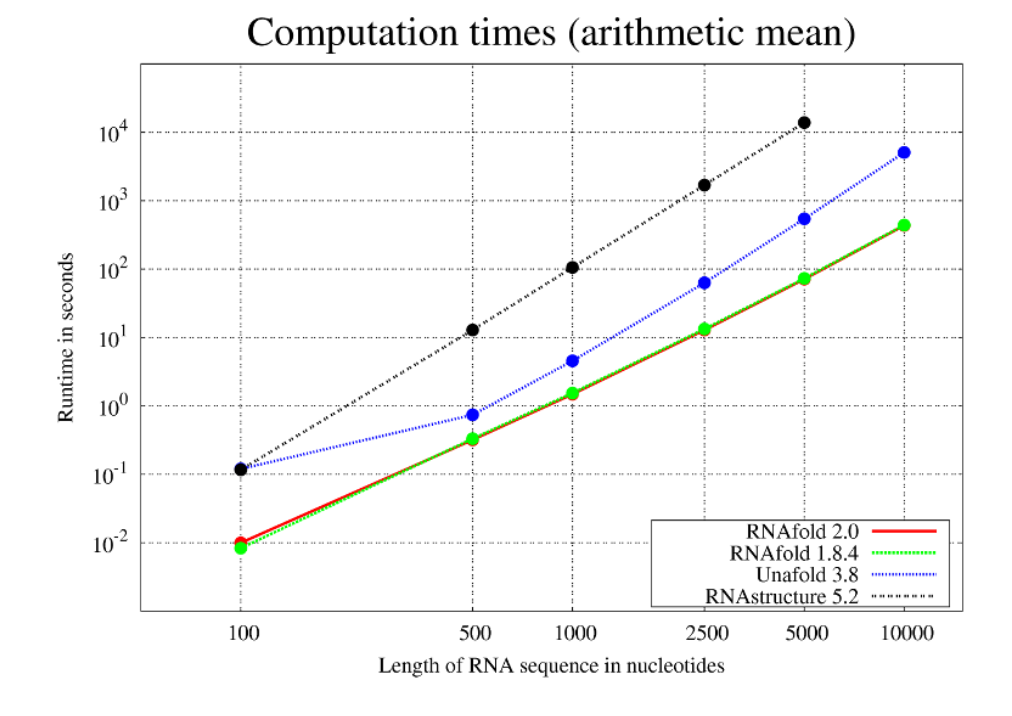
\includegraphics[width=\textwidth]{../img/rnafold}
\caption{Výsledky analýzy dĺžky behu programu RNAfold, v závislosti na dĺžke sekvencie predikovanej sekundárnej štruktúry. Obrázok bol 13.07.2019 stiahnutý z \url{https://www.tbi.univie.ac.at/RNA/}.}
\label{obr5.15}
\end{figure}


\section{Experiment a Výsledky}
Za účelom overenia vplyvu pridania predikcie sekundárnej štruktury do pôvodného algoritmu sme urobili rovnaké testovanie nad rovnakými dátami, ako pri porovnávaní pôvodného algoritmu s ModeRNA \autoref{ModeRNA}. Skúšali sme napredikovať všetky páry s podobnosťou medzi 60\% - 90\% a dĺžkou 50-100 a 101-500 nukleotidov najprv pôvodnou verziou algoritmu Trooper, verziou algoritmu vylepšenou o predikciu sekundárnej štruktúry a referenčnou predikciou ModeRNA. 


\indent  Výsledky a porovnanie predikcií uvádzame v tabuľke \autoref{tab5.1}. Z výsledkov vidíme, že pridanie predikcie sekundárnej štruktúry spôsobilo, že priemerná RMSD pre štruktúry s dĺžkou medzi 50-100 nukleotidov na 413 úspešne napredikovaných pároch sa zhoršila z 5,80Å na 8,23Å, čo približne zodpovedá výsledku 8,53Å, ktoré na predikcii rovnakých štruktúr dosiahla ModeRNA. Pri predikcii štruktúr dĺžky 101-500 nukleotidov a 98 úspešne napredikovaných pároch sa naopak priemerné výsledky predikcie s pridaním predikcie sekundárnej štruktýry výrazne zlepšili a to z 6,91Å na 3,46Å, čo je o niečo lepšie než výsledky ModeRNA, ktorá pri rovnakých podmienkach dosiahla priemer 3,72Å. 
\begin{table}[b!]
\centering
\begin{tabular}{ccccc}
\toprule
Veľkosť & Počet párov & Trooper bez SS & Trooper s SS & ModeRNA\\
\midrule
50-100  & 413 & 5,80  & 8,23 & 8,53\\
101-500  & 98 & 6,91  & 3,46 & 3,72\\
\bottomrule
50-500  &  511 & 5,95  & 7,31 & 7,61\\
\end{tabular}
\caption{Porovnanie priemernej RMSD predikcie RNA nástrojmi Trooper, Trooper s predikciou sekundárnej štruktúry a ModeRNA. }\label{tab5.1}
\end{table}


\indent Z výsledkov je teda zrejmé, že pridanie predikcie sekundárnej štruktúry a jej poskytnutie algoritmu FARFAR v niektorých prípadoch výsledky zlepšilo a v niektorých zhoršilo. Prečo boli zlepšené práve dlhšie štruktúry by sme mohli vysvetliť tak, že dlhšie štruktúry môžu obsahovať dlhšie nekonzervované úseky, ktorých predikcia je pre FARFAR náročnejšia. Príklad z obrázka \autoref{obr5.1} práve podporuje takúto teóriu, kedy vidíme, že pôvodná predikcia FARFAR bez sekundárnej štruktúry napredikovala nekonzervovaný úsek zle, ale po pridaní sekundárnej štruktúry sa FARFAR-u podarilo úsek napredikovať oveľa presnejšie.
\begin{figure}%[p]\centering
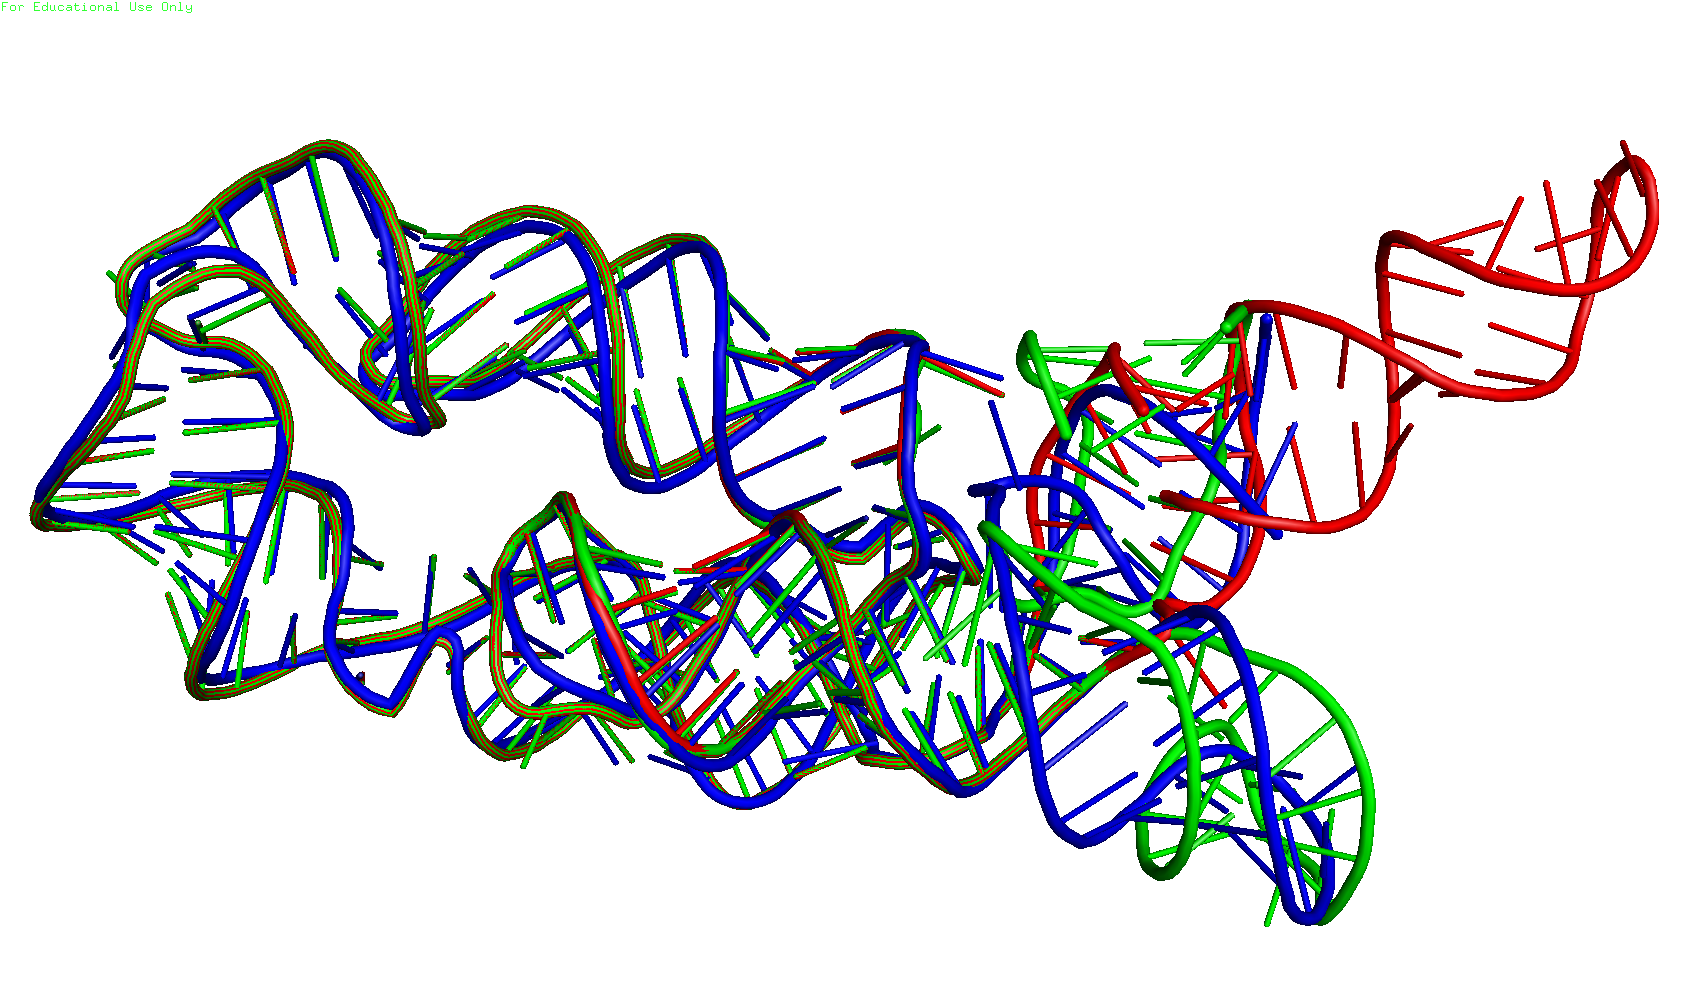
\includegraphics[width=\textwidth]{../img/struct1}
\caption{Modrá štruktúra je experimentálne získana štruktúra molekuly 3DIG:X s dĺžkou 175 nukleotidov. Červená štruktúra je predikovaná algoritmom Trooper bez použitia sekundárnej štruktúry s výslednou RMSD na úrovni 14,44Å. Zelená štruktúra je predikcia urobená algoritmom Trooper s výslednou RMSD 4,44Å. Pre obe predikcie bol použitý rovnaký template, a to štruktúra 3DOU:A.}
\label{obr5.1}
\end{figure}


\indent Ďalej sme ešte skúmali značné zhoršenie výsledkov v triede štruktúr veľkostí 50-100 nukleotidov z RMSD 5,8Å na 8,23Å. Zastávame hypotézu, že by to mohlo byť spôsobené nesprávnou sekundárnou štruktúrou dodanou algoritmu FARFAR, pretože inak boli podmienky oboch predikcií rovnaké, a teda by sa priemerné výsledky nemali od seba značne líšiť.


\indent Správnosť predikovanej sekundárnej štruktúry vieme popísať a klasifikovať štyrma mierami: true positives (správne určený existujúci base-pair), true negatives (správne určený nespárovaný nukleotid), false positives (nesprávne určený base-pair) a nakoniec false negative (v štruktúre by mal existovať base-pair, ale nie je napredikovaný). Z týchto štyroch ukazateľov sú prvé dva pozitívne a druhé dva negatívne. Pritom ale FARFAR-u môže uškodiť iba prípad false negative, pretože ten mu indikuje, že má v predikcii spárovať (a teda umiestniť blízko seba) dva nukleotidy. Prípady s false negatives by predikciu FARFAR-u nemali zlepšiť, ale ani zhoršiť, pretože nekladú žiadnu podmienku na spárovanie nukleotidov. 


\indent Zamerali sme sa preto na prípady false positives v predikovaných sekundárnych štruktúrach a analyzovali sme koreláciu medzi zhoršením, prípadne zlepšením predikcie algoritmu Trooper bez sekundárnej štruktúry a algoritmu Trooper s predikciou sekundárnej štruktúry vzhľadom na počet false positives v napredikovanej sekundárnej štruktúre dodanej ako vstup algoritmu FARFAR. Výsledok je graficky znázornený na obrázku \autoref{obr5.2} a podporuje našu hypotézu o tom, že čím viac vzrastal počet false positives v predikovanej sekundárnej štruktúre, tým bolo pravdepodobnejšie, že predikcia so sekundárnou štruktúrou sa oproti predikcii bez sekundárnej štruktúry zhorší. Preto si myslíme, že zhoršenie v niektorých preikciách bolo spôsobené hlavne zle napredikovanou sekundárnou štruktúrou.
\begin{figure}%[p]\centering
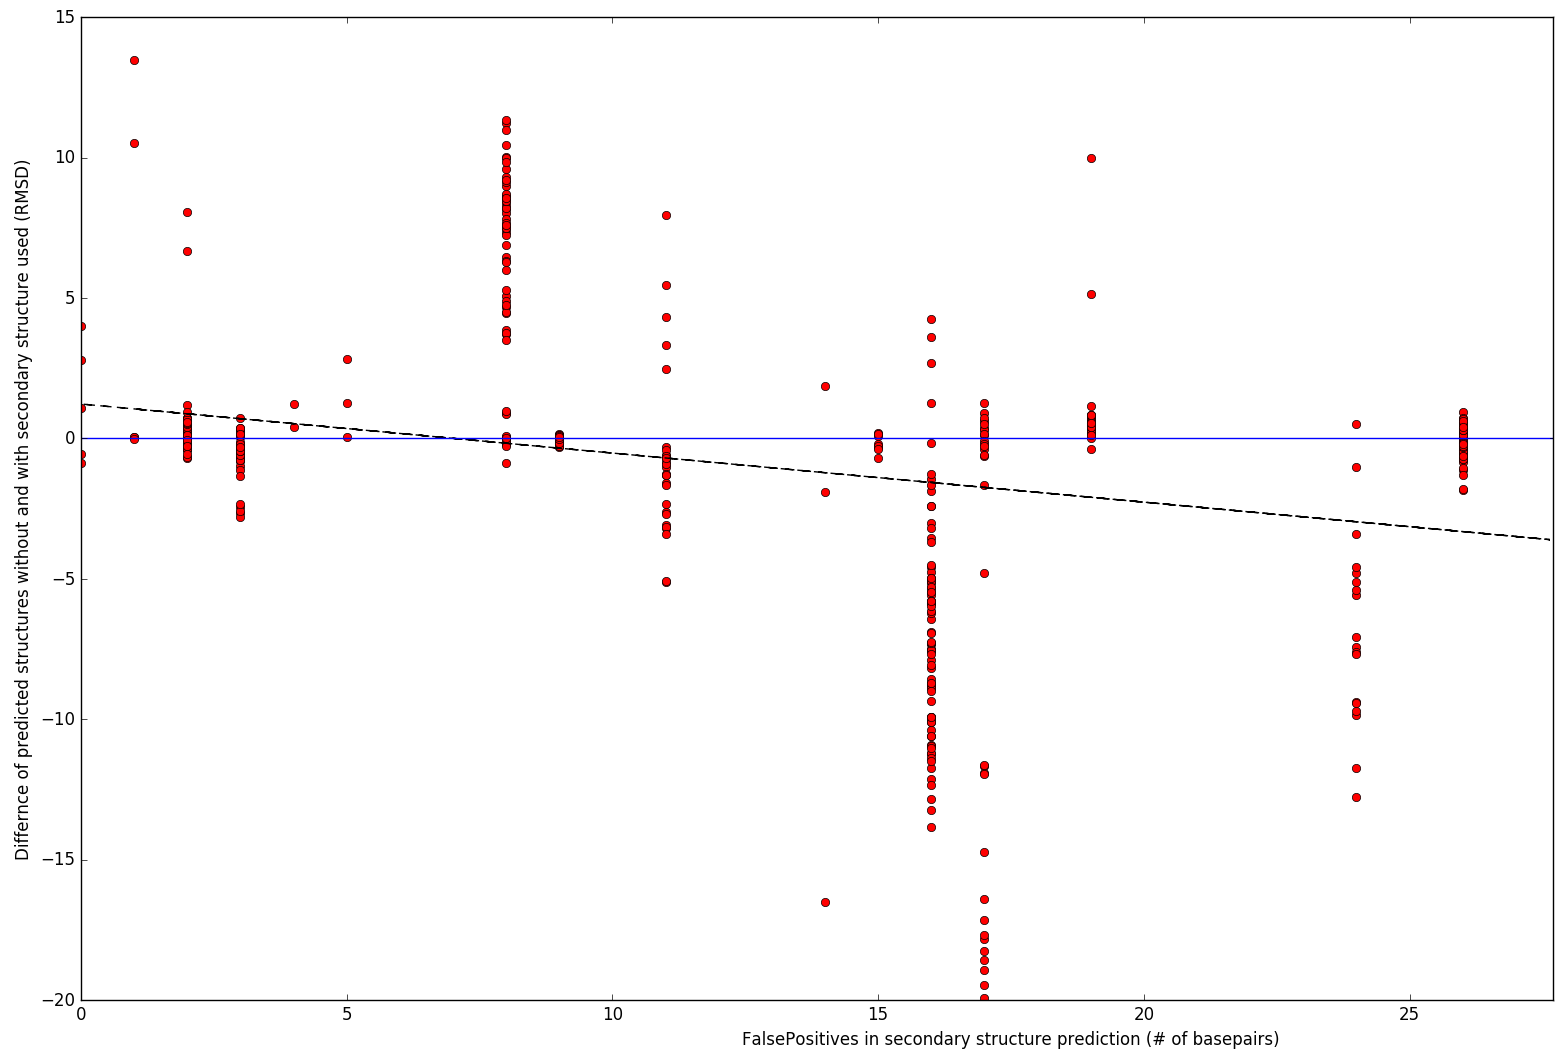
\includegraphics[width=\textwidth]{../img/corelation}
\caption{Závislosť medzi rozdielom výsledkov predikcie s a bez sekundárnej štruktúry a počtom false positive base-pairs v napredikovanej sekundárnej štruktúre. Červené body sú jednotlivé záznamy a čiarkovanou čiarou je zobrazená lineárna regresia týchto bodov.}
\label{obr5.2}
\end{figure}
\chapter{Použitie viacerých template štruktúr pri predikcií}

Ako druhé opatrenie, na zlepšenie rýchlosti a presnosti predikovania nekonzerovvaných úsekov sme navrhli skúsiť použiť viacero template štruktúr na predikciu jednej template štruktúry. Očakávali sme pritom, že sa nám podarí zmenšiť počet a dĺžku nekonzervovaných úsekov v predikovanej štruktúre a tým výrazne zjednosušiť ich predikciu algoritmom FARFAR.

\section{Varianty a prístupy}


\section{Výber vhodných štruktúr}


\section{Algoritmus}


\section{Integrácia do existujúceho algoritmu}


\section{Experiment}


\section{Výsledky}

\chapter*{Závěr}
\addcontentsline{toc}{chapter}{Závěr}
Primárnym cieľom tejto práce bolo rozšíriť pôvodný algoritmus predikcie terciárnej štruktúry za pomoci vzorovej štruktúry o dva moduly, ktoré by zlepšili problematickú predikciu štruktúr obsahujúcich dlhé nekonzervované úseky. Okrem toho sme chceli predikciu zautomatizovať tak, aby nevyžadovala manuálne zásahy, a následne naše výsledky porovnať s algoritmom ModeRNA.

\indent Prvý modul, ktorý vkladá do predikcie terciárnej štruktúry medzikrok predikcie sekundárnej štruktúry, sme úspešne navrhli, implementovali a otestovali. Z testovania vyplynulo, že časť predikovaných štruktúr sa zlepšila a časť naopak zhoršila, za čo, ako sme analýzou ukázali, môžu hlavne nepresne napredikované sekundárne štruktúry target molekuly.
Návrh druhého modulu, pomocou ktorého vieme pri predikcii jednej target štruktúry použiť viacero template štruktúr, sa ukázal byť zložitejší. Prvé dva návrhy algoritmu sa pri testovaní ukázali ako nepoužiteľné, ale tretiu verziu algoritmu sa nám podarila naimplementovať a odladiť do takej miery, že sme boli schopní získať výsledky indikujúce, že pri nájdení správnej sekundárnej template štruktúry sme schopní výsledok predikcie zlepšiť, ale naopak pri použití nevhodnej štruktúry sa môžu výsledky výrazne zhoršiť.
Implementáciu algoritmu sa nám podarilo úspešne automatizovať do takej miery, že na hromadnú predikciu štruktúr a vyhodnotenie výsledkov stačí spustiť štyri shell skripty. Vďaka tomu sme dokázali výsledky algoritmu Trooper porovnať s výsledkami algoritmu ModeRNA, pričom sa ukázalo, že náš algoritmus bol vo verzii so sekundárnou štruktúrou v celkovom priemere RMSD o niečo presnejší.  

  
\indent Výsledky našej práce ukázali, že obe metódy majú potenciál, aby pri použití správnej sekundárnej štruktúry, alebo ďalšej vhodnej template štruktúy, dokázali výsledky predikcie zlepšiť. Okrem toho sme ukázali, že naše aktuálne výsledky sú porovnateľné s konkurenčným algoritmom ModeRNA.
V budúcnosti by sme sa práve chceli zamerať na zlepšenie predikcie sekunárnych štruktúr a ďalšie vyladenie hľadania vhodných template štruktúr. Takisto by sme chceli zbaviť nášu implementáciu závislosti na algoritme FARFAR a predikciu nekonzervovaných úsekov zabezpečovať vlastným riešením.

%%% Seznam použité literatury
%%% Seznam použité literatury (bibliografie)
%%%
%%% Pro vytváření bibliografie používáme bibTeX. Ten zpracovává
%%% citace v textu (např. makro \cite{...}) a vyhledává k nim literaturu
%%% v souboru literatura.bib.
%%%
%%% Příkaz \bibliographystyle určuje, jakým stylem budou citovány odkazy
%%% v textu. V závorce je název zvoleného souboru .bst. Styly plainnat
%%% a unsrt jsou standardní součástí latexových distribucí. Styl czplainnat
%%% je dodáván s touto šablonou a bibTeX ho hledá v aktuálním adresáři.

\bibliographystyle{czplainnat}    %% Autor (rok) s českými spojkami
% \bibliographystyle{plainnat}    %% Autor (rok) s anglickými spojkami
% \bibliographystyle{unsrt}       %% [číslo]

\renewcommand{\bibname}{Seznam použité literatury}

%%% Vytvoření seznamu literatury. Pozor, pokud jste necitovali ani jednu
%%% položku, seznam se automaticky vynechá.

\bibliography{literatura}

%%% Kdybyste chtěli bibliografii vytvářet ručně (bez bibTeXu), lze to udělat
%%% následovně. V takovém případě se řiďte normou ISO 690 a zvyklostmi v oboru.

% \begin{thebibliography}{99}
%
% \bibitem{lamport94}
%   {\sc Lamport,} Leslie.
%   \emph{\LaTeX: A Document Preparation System}.
%   2. vydání.
%   Massachusetts: Addison Wesley, 1994.
%   ISBN 0-201-52983-1.
%
% \end{thebibliography}


%%% Obrázky v diplomové práci
%%% (pokud jich je malé množství, obvykle není třeba seznam uvádět)
\listoffigures

%%% Tabulky v diplomové práci (opět nemusí být nutné uvádět)
%%% U matematických prací může být lepší přemístit seznam tabulek na začátek práce.
\listoftables

%%% Použité zkratky v diplomové práci (opět nemusí být nutné uvádět)
%%% U matematických prací může být lepší přemístit seznam zkratek na začátek práce.
%\chapwithtoc{Seznam použitých zkratek}

%%% Přílohy k diplomové práci, existují-li. Každá příloha musí být alespoň jednou
%%% odkazována z vlastního textu práce. Přílohy se číslují.
%%%
%%% Do tištěné verze se spíše hodí přílohy, které lze číst a prohlížet (dodatečné
%%% tabulky a grafy, různé textové doplňky, ukázky výstupů z počítačových programů,
%%% apod.). Do elektronické verze se hodí přílohy, které budou spíše používány
%%% v elektronické podobě než čteny (zdrojové kódy programů, datové soubory,
%%% interaktivní grafy apod.). Elektronické přílohy se nahrávají do SISu a lze
%%% je také do práce vložit na CD/DVD. Povolené formáty souborů specifikuje
%%% opatření rektora č. 72/2017.
\appendix
%\chapter{Přílohy}

%\section{První příloha}

\openright
\end{document}
